%!TEX root = ../aluno.tex

\chapter{Juntando frações da unidade}

\null\vfill
\begin{figure}[H]
\centering
% \begin{tikzpicture}
% \sethlcolor{white}
% \tikzset{x=1mm, y=1mm}
% \tikzstyle{fala}=[rectangle, fill=white]
% \linespread{.7}
% \node [anchor=center] at (0,0){
% 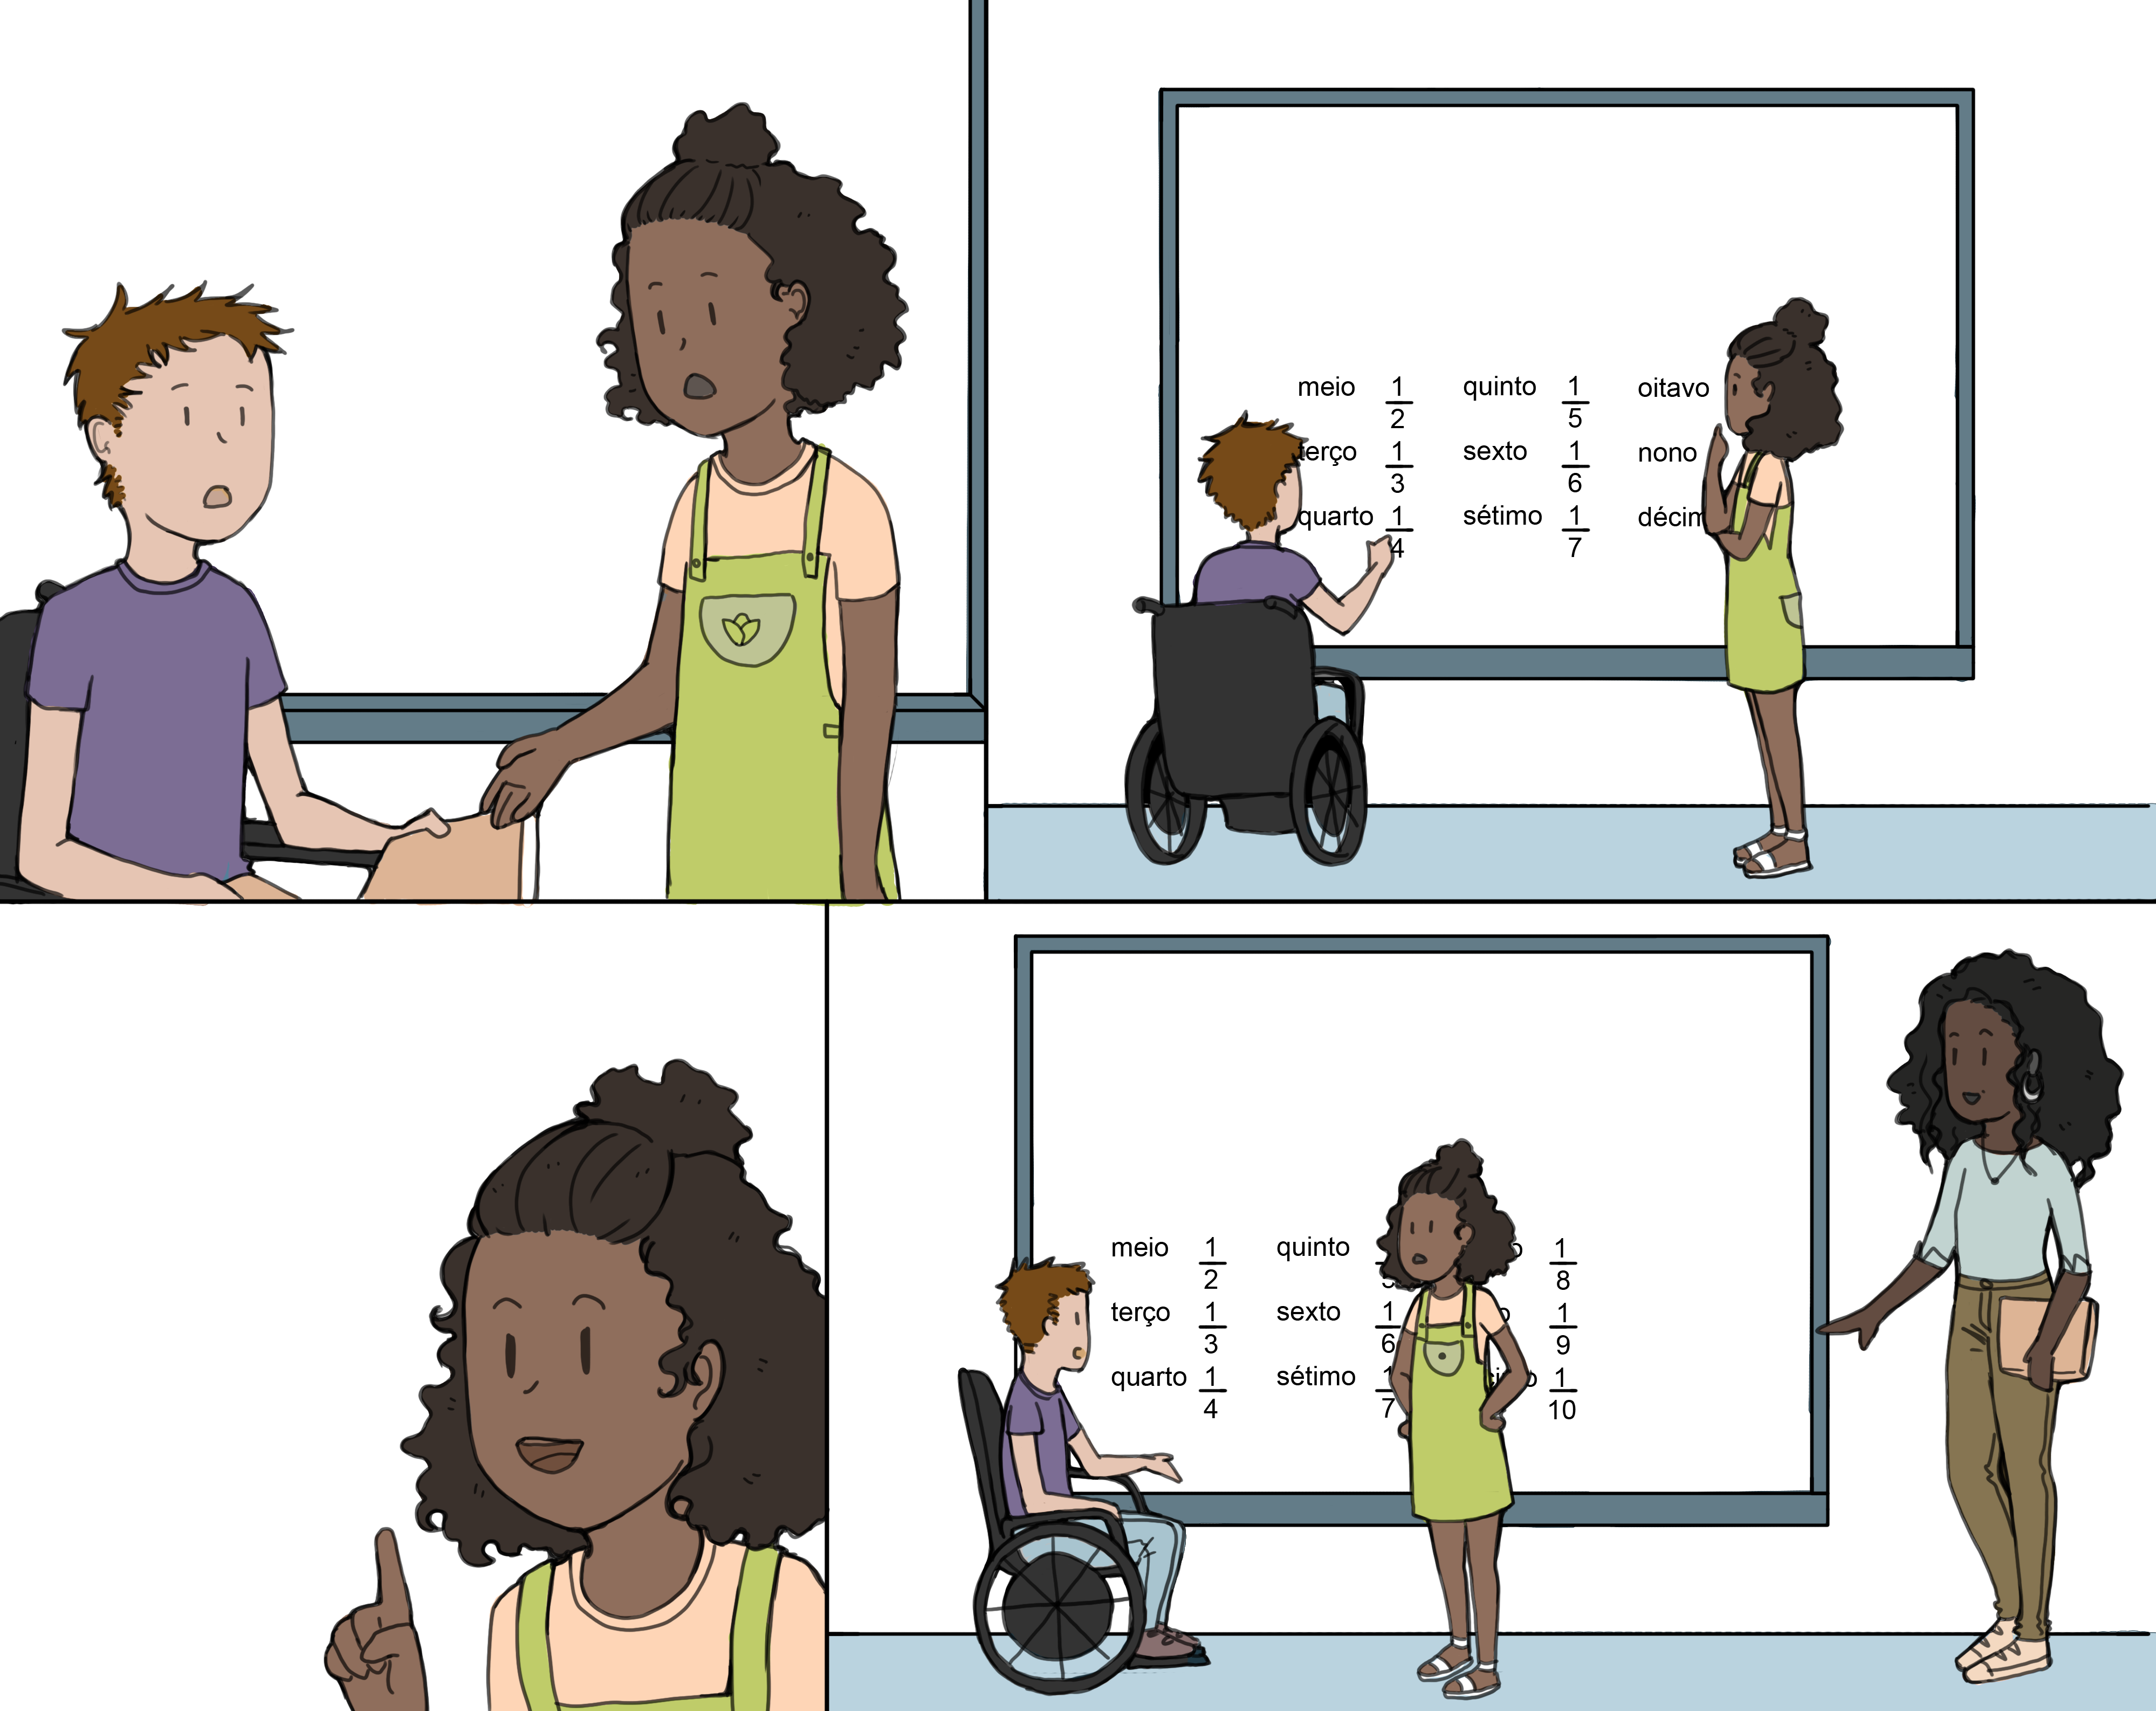
\includegraphics[width=.96\textwidth, keepaspectratio]{licao02/quadrinho-licao2-agnes.png}
% };
% \node [fala, text width=5.5cm,align=justify] at (-45,62.5) {\tiny Oi Miguel, por que você faltou a aula passada? A professora falou de frações. \\ Recortamos papéis em partes iguais.};

% \node [fala, text width=4cm,align=justify] at (-57.6,45) {\tiny Eu tive febre. Mas minha mãe me ensinou frações em casa.};


% \node [fala, text width=4cm,align=justify] at (17.5,40) {\tiny Tem o meio, o um terço, o um quarto etc. até o um décimo.};

% \node [fala, text width=5.5cm,align=justify, fill=white] at (50,57.5) {\tiny Não foi bem isso que vimos. Depois de repartir as figuras em partes iguais ou de mesma forma, cada uma delas recebeu um desses nomes.};

% \node [text width=5.5cm,align=justify] at (-49,-12) {\tiny Esse negócio não parece estar certo. Os números ficam um ao lado do outro: treze, quatorze, quinze.... E não um \hl{embaixo do} outro como você mostrou aí!};

% \node [fala, text width=4.75cm,align=justify] at (32.5,-12.5) {\tiny Crianças, não briguem. Vamos ver frações em símbolos matemáticos na aula de hoje.};

% % \draw [] (40,-17) -- (55,-17);
% \end{tikzpicture}

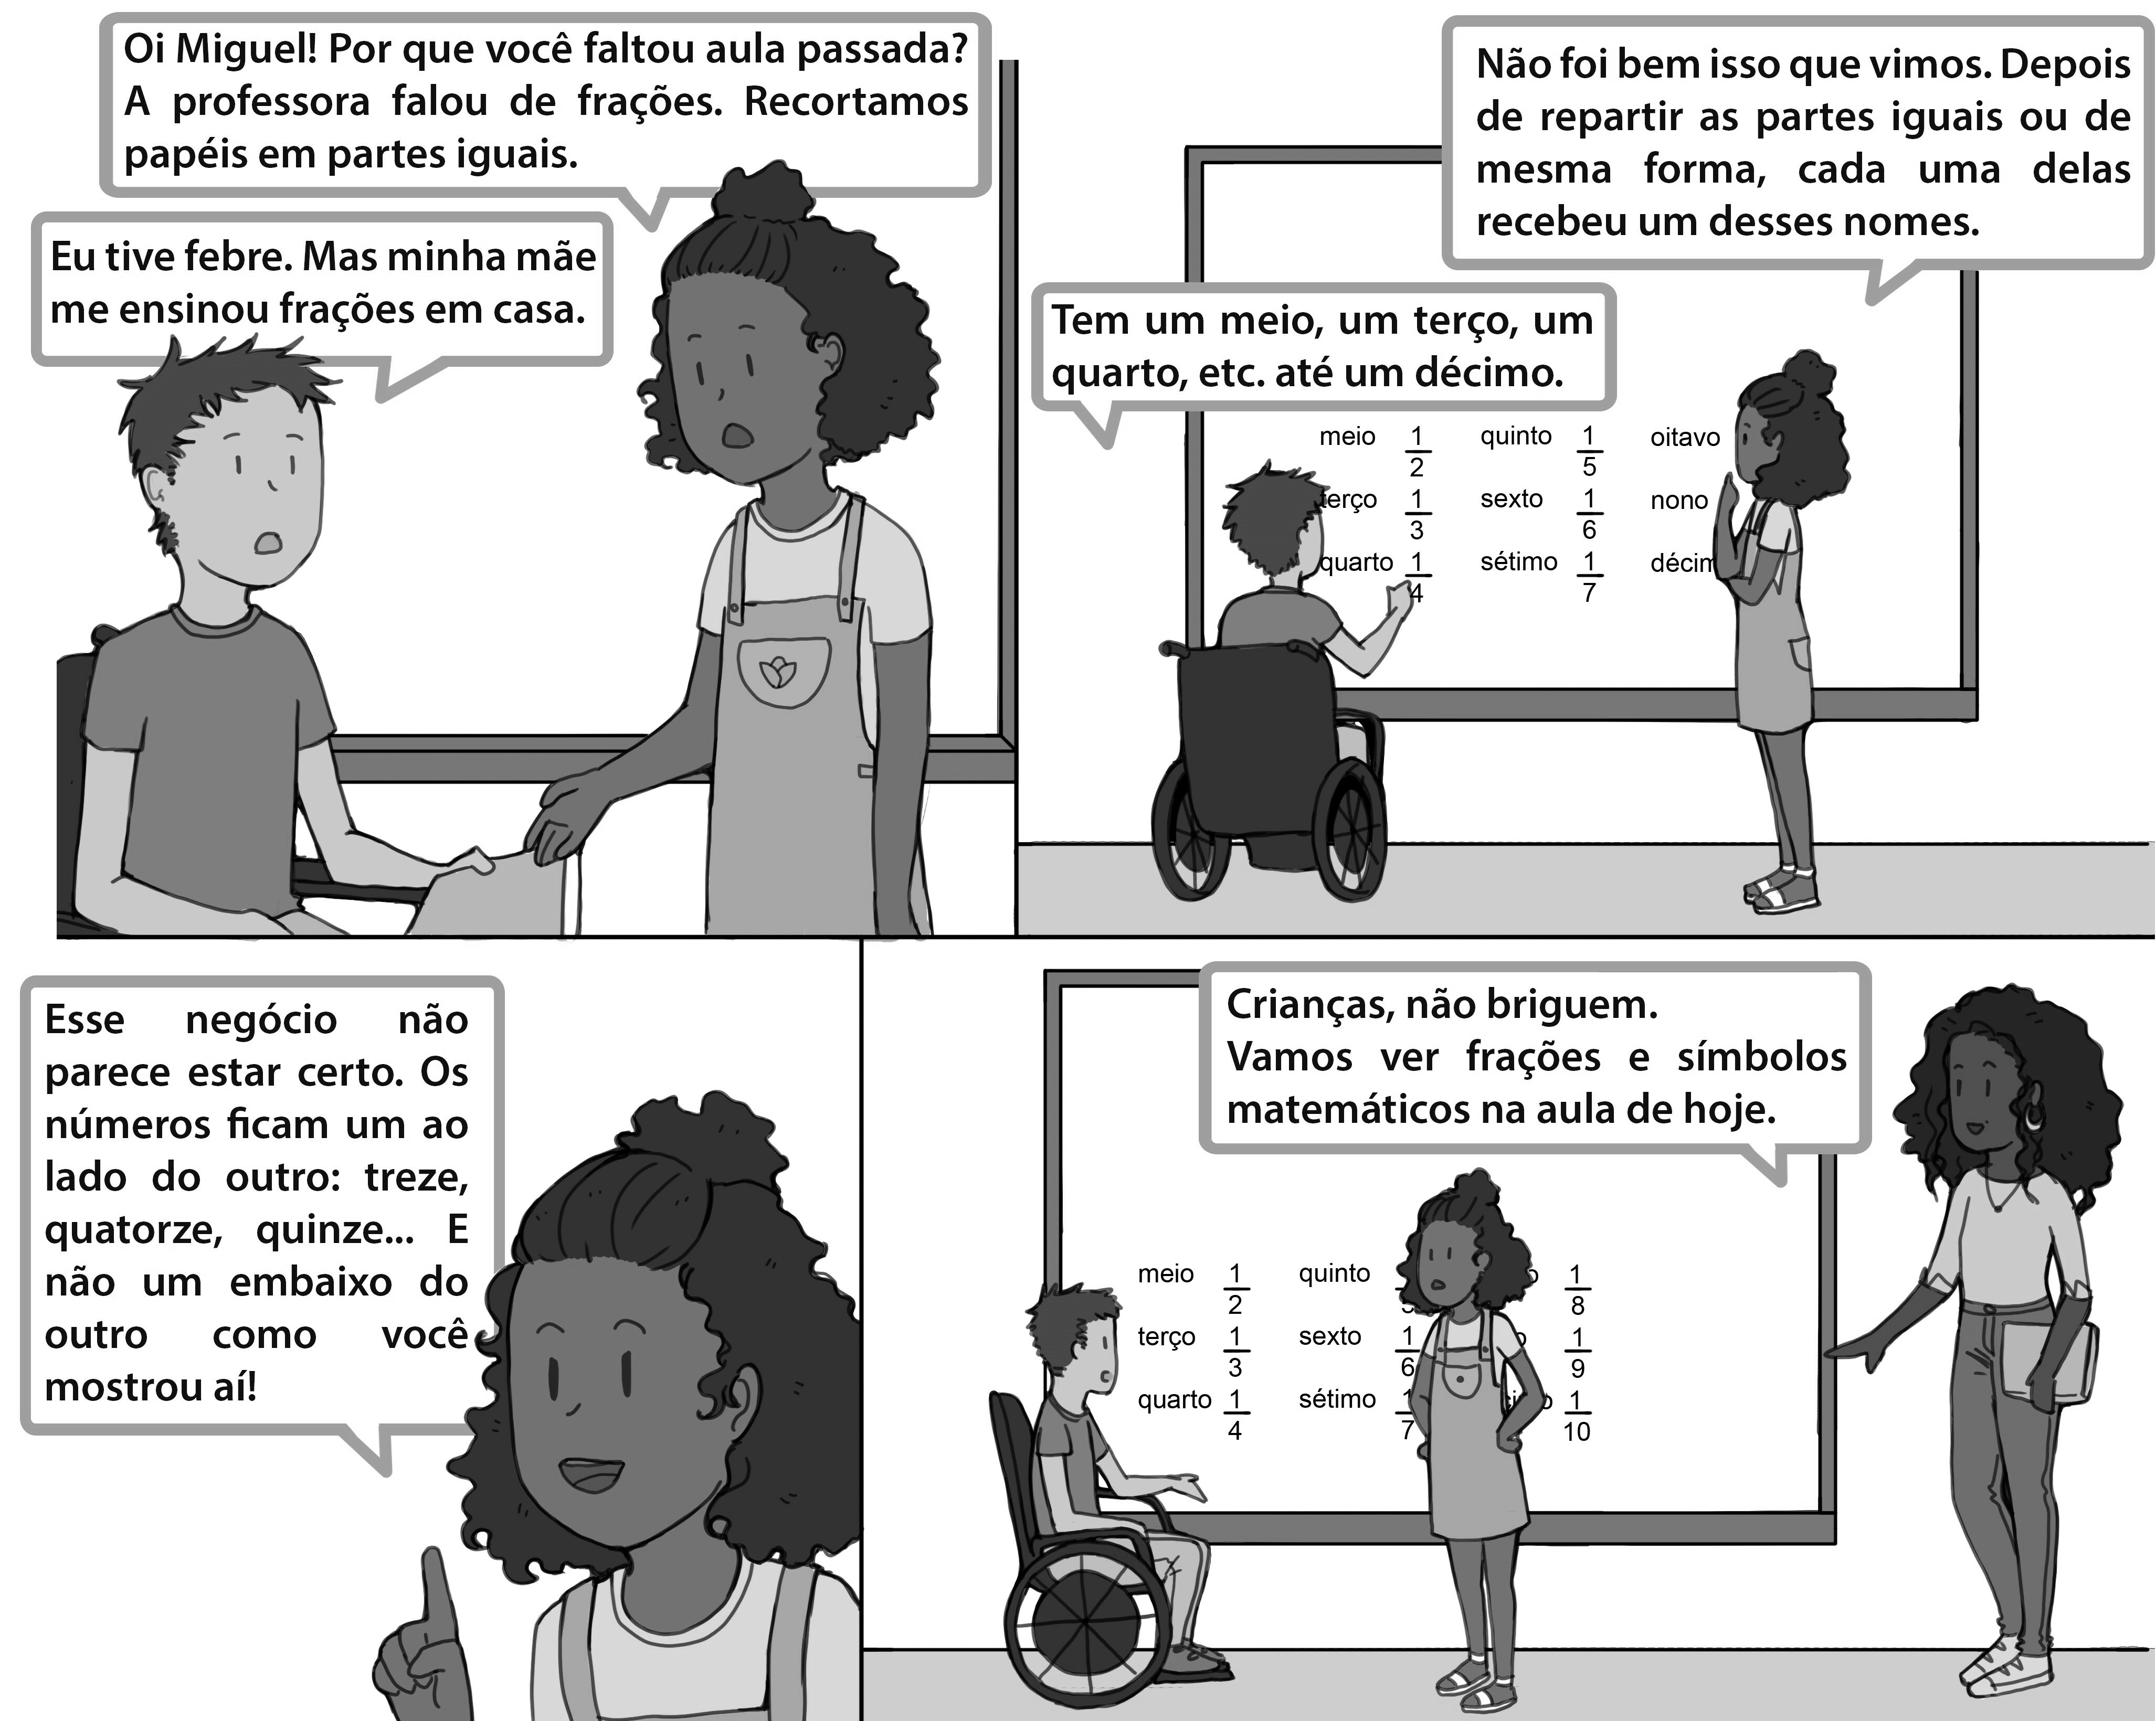
\includegraphics[width=\textwidth, keepaspectratio]{licao02/quadrinho-licao2-agnes}
\end{figure}
\vfill\null
\newpage

\section{Explorando o Assunto}

\begin{atividade}{}\label{chap2-ativ1}

Luiza, João e Mariele foram a uma pizzaria. Cada um pediu uma pizza do seu sabor preferido. 
Luiza cortou sua pizza em 4 fatias; João cortou sua pizza em 6 fatias e Mariele cortou sua pizza em 8 fatias.

%Veja o quanto restou de pizza após os amigos estarem satisfeitos:
O esquema a seguir indica o quanto restou de pizza após os amigos estarem satisfeitos:

\begin{center}
\begin{tikzpicture}[scale=.8]
\draw [dashed] (0,0) circle (2cm);
\filldraw[fill=common] (0,0) -- (120: 2cm) arc (120:240:2cm)--cycle;
\foreach \t in {0,60,300}{
  \draw [dashed] (0,0) -- (\t: 2cm);
}
\draw (0,0) -- (180:2cm);
\end{tikzpicture}\hspace{2cm}
\begin{tikzpicture}[scale=.8]
\draw [dashed] (0,0) circle (2cm);
  \filldraw[fill=common] (0,0) -- (135: 2cm) arc (135:225:2cm)--cycle;

\foreach \t in {0,45,...,315}{
  \draw [dashed] (0,0) -- (\t: 2cm);
}
\draw  (0,0) -- (135: 2cm);
\draw  (0,0) -- (180: 2cm);
\draw  (0,0) -- (225: 2cm);
\end{tikzpicture}\hspace{2cm}
\begin{tikzpicture}[scale=.8]
\draw [dashed] (0,0) circle (2cm);
  \filldraw[fill=common] (0,0) -- (180: 2cm) arc (180:270:2cm)--cycle;

\foreach \t in {0,90}{
  \draw [dashed] (0,0) -- (\t: 2cm);
}
\draw (0,0) -- (180: 2cm);
\draw (0,0) -- (270: 2cm);
\end{tikzpicture}
\end{center}

\begin{enumerate}  %d
\item   Identifique a pizza de cada um dos amigos.
\item   Em cada caso, que fração da pizza representa uma fatia?
\item   Escreva a quantidade de pizza que cada amigo comeu utilizando fração?
\end{enumerate}
 \end{atividade}


\begin{atividade}{}\label{chap2-ativ2}

O pai de Ana, Beatriz e Clara trouxe duas barras de chocolate para serem repartidas entre elas.

\begin{center}
\begin{tikzpicture}[x=1mm,y=1mm, scale=0.9]
\draw[fill=chocolate] (0,0) rectangle (60,20);
\draw[fill=chocolate, shift={(75,0)}] (0,0) rectangle (60,20);
\end{tikzpicture}
\end{center}

Ana propôs que cada barra fosse dividida em três partes iguais e que cada irmã ficasse com duas dessas partes.

\begin{center}
\begin{tikzpicture}[x=1mm,y=1mm,scale=0.9]
%%%%%%%%%% espaço entre um início de barra repartida e outro.
\def\hsp{150} 
%%%%%%%%%% barras de chocolate
\draw[fill=chocolate](0,10) rectangle (60,30);
\draw[fill=chocolate] (0,-15) rectangle (60,5);

%%%%%%%%% cortes
\draw[dashed, thick] (20,35) -- (20,-20);
\draw[dashed, thick] (40,35) -- (40,-20);

%%%%%%%%% setas
\draw[very thick, ->] (10,-17) -- (-20,-27);
\draw[very thick, ->] (30,-17) -- (30,-27);
\draw[very thick, ->] (50,-17) -- (80,-27);

\node at (95,-20) {\parbox[b]{30mm}{\centering  \small Sugestão da Ana}};

%%%%%%%%%%%%%%%%%%Pedaços repartidos  
\draw[fill=chocolate,xshift=-\hsp] (20,-50) rectangle (40,-30);
\draw[fill=chocolate,xshift=-\hsp] (20,-75) rectangle (40,-55);

\draw[fill=chocolate] (20,-50) rectangle (40,-30);
\draw[fill=chocolate] (20,-75) rectangle (40,-55);

\draw[fill=chocolate,xshift=\hsp] (20,-50) rectangle (40,-30);
\draw[fill=chocolate,xshift=\hsp] (20,-75) rectangle (40,-55);

%%%%%%%%% Texto embaixo
% \draw [thick, decoration={brace,mirror,raise=5}, decorate, xshift=-\hsp] (31.25,-2) -- (51.25,-2) node [pos=0.5,anchor=north,yshift=-10] {\parbox[b]{40mm}{\centering Quantidade de chocolate recebida por Ana}};

\node [xshift=-\hsp, text width=50mm, align=center] at (30,-87) {\centering \small Quantidade de chocolate recebida por Ana};

\node [text width=50mm, align=center] at (30,-87) {\small Quantidade de chocolate recebida por Beatriz};

\node  [xshift=\hsp, text width=50mm, align=center] at (30,-87) {\centering  \small Quantidade de chocolate recebida por Clara};

%%%%%%%%%%%% Balões em volta
% \draw [dotted, xshift=-\hsp] (30,-52.5) ellipse (20mm and 30mm);
% \draw [dotted] (30,-52.5) ellipse (20mm and 30mm);
% \draw [dotted, xshift=\hsp] (30,-52.5) ellipse (20mm and 30mm);
\end{tikzpicture}
\end{center}

\begin{enumerate} %s
  \item Na divisão de cada uma das barras de chocolate em três partes iguais, ca\-da parte é que fração de uma barra de chocolate?
  \item Você concorda com a divisão que Ana sugeriu? Explique.
  \item Com essa divisão, as três irmãs receberam a mesma quantidade de chocolate?
  \item Na divisão proposta por Ana, como você nomearia, usando fração de uma barra de chocolate, a quantidade de chocolate que cada irmã recebeu?
\end{enumerate}

Ana não quer o chocolate e decidiu dar a quantidade de chocolate que recebeu na divisão das barras para as suas irmãs.

\begin{enumerate}\setcounter{enumi}{4}
\item Se Ana desse metade da quantidade de chocolate que recebeu para cada uma de suas irmãs, que quantidade de chocolate Beatriz e Clara passariam a ter? Como você nomearia, usando frações, essas quantidades?
\item E se Ana desse toda a quantidade de chocolate que recebeu para Beatriz, que quantidade de chocolate  Beatriz passaria a ter? Como você nomearia, usando frações, essa quantidade?
\end{enumerate} %s
\end{atividade}

\begin{atividade}{}\label{chap2-ativ3}
\tikzset{x=1cm,y=1cm}

Um grupo de cinco amigos (Amarildo, Beto, Carlos, Davi e Edilson) encomendou três tortas salgadas, de mesmo tamanho retangular, como na ilustração para uma comemoração.

\begin{center}
 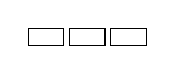
\begin{tikzpicture}[scale=0.75]
  \draw (0,0) rectangle (6,3);
  \draw (7,0) rectangle (13,3);
  \draw (14,0) rectangle (20,3);
 \end{tikzpicture}

\end{center}

\begin{enumerate}  %s
  \item     Como dividir as três tortas de modo que cada amigo receba a ~ mesma quantidade de torta? Faça um desenho no seu caderno mostrando sua proposta de divisão. Indique qual parte é de qual amigo!
  \item     Considerando-se uma torta como unidade, como você nomearia, usando frações, a quantidade de torta que:
\begin{enumerate}[label=\textbf{\roman*)}, left=1em] %d
      \item         Amarildo recebeu?
      \item         Amarildo e Beto receberam juntos?
      \item         Amarildo, Beto e Carlos receberam juntos?
      \item         Amarildo, Beto, Carlos e Davi receberam juntos?
      \item         Amarildo, Beto, Carlos, Davi e Edilson receberam juntos?
\end{enumerate} %d

  \item     A quantidade de torta que cada amigo recebeu é menor do que um quinto de torta? E do que dois quintos de torta? Explique sua resposta.
  \item     A quantidade de torta que cada amigo recebeu é maior do que três quintos de torta? E do que quatro quintos de torta? Explique sua resposta.
\end{enumerate} %s
\end{atividade}

\begin{atividade}{}\label{chap2-ativ4}

Para a sobremesa do almoço de domingo, papai passou em uma confeitaria que vende tortas.
Cada torta está dividida em  igualmente em 8 fatias, como na figura abaixo.

\begin{center}
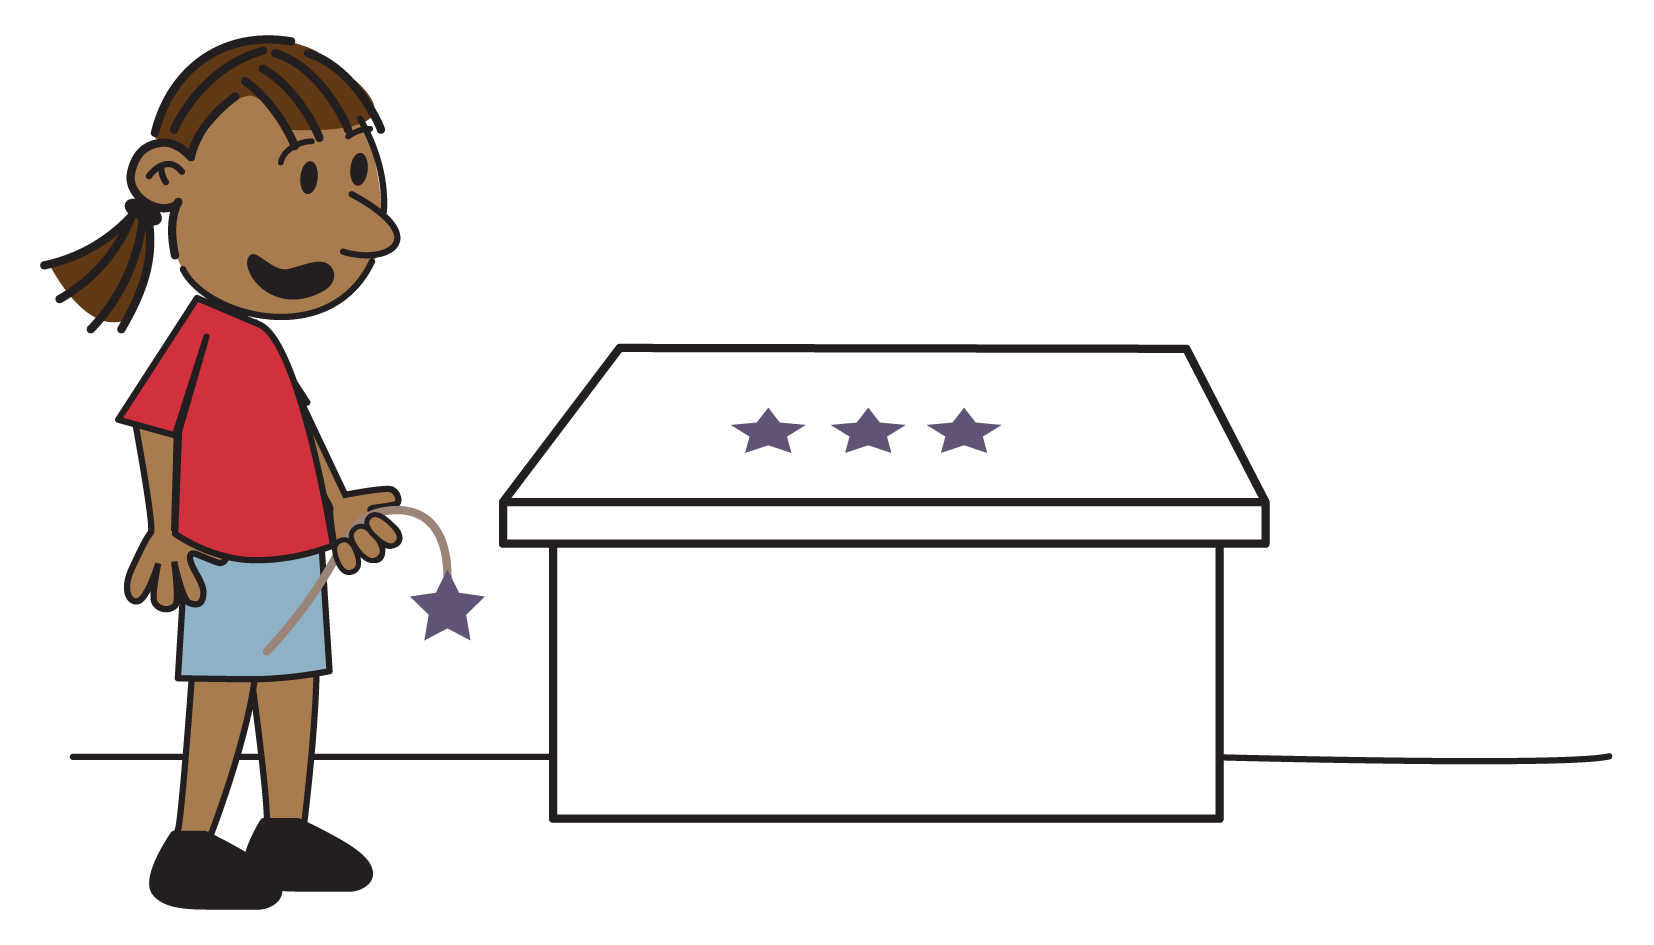
\includegraphics[width=.5\textwidth, keepaspectratio]{licao02/ativ3_fig01.png}
\end{center}

\begin{enumerate}  %s
  \item     Que fração de uma torta é uma fatia? Explique.
  \item     Domingo papai comprou 4 fatias, quantos oitavos de uma torta havia para a sobremesa?
  \item     Na pergunta anterior, apresente outra fração que represente a quantidade de torta que papai comprou. Explique sua resposta.
  \item     Hoje papai comprou 10 fatias de torta. Como podemos representar essa quantidade de torta em termos de frações de uma torta?
\end{enumerate} %s
\end{atividade}

\begin{atividade}{}\label{chap2-ativ5}
\tikzset{x=1mm,y=1mm}

Complete as afirmações com uma das frações: ``dois meios'', ``dois terços'', ``dois quintos'', ``dois nonos'', ``três quartos'', ``seis oitavos'', ``oito sextos'' e ``no\-ve meios'', para que sejam verdadeiras.

\begin{enumerate}
\item A parte em destaque em
     \begin{tikzpicture}[scale=0.8]
     \draw[fill=attention] (0,0) rectangle (20,10);
     \draw[] (10,0) -- (10,10);
     \draw[fill=common, fill opacity=.3] (20,0) rectangle (30,10);
     \end{tikzpicture}
     é
\hrulefill
     de \begin{tikzpicture}[scale=0.8]
     \draw[fill=common, fill opacity=.3] (0,0) rectangle (30,10);
                               \end{tikzpicture}.
\item A parte em destaque em \begin{tikzpicture}
                           \draw[fill=attention] (0,0) rectangle (8,8);
                           \draw (0,0) -- (8,8);
                          \end{tikzpicture}
                          é \hrulefill
                            de \begin{tikzpicture}
                            \draw[fill=common, fill opacity=.3] (0,0) rectangle (8,8);
                           \end{tikzpicture}.


 \item A parte em destaque em \begin{tikzpicture}
                           \draw[fill=common, fill opacity=.3] (0,0) circle (4);
                           \fill[attention] (0,0) -- (72:4) arc (72:-72:4) --cycle;
                           \foreach \x in {0,72,...,288}{
                           \draw (0,0) -- (\x:4);}
                          \end{tikzpicture}
                          é \hrulefill
                            de \begin{tikzpicture}
                            \draw[fill=common, fill opacity=.3] (0,0) circle (4);
                           \end{tikzpicture}.

 \item A parte em destaque em 
 \tikzset{x=.8mm, y=.8mm}
 \begin{tikzpicture}
\fill[attention]  \foreach \x/\y in {36/72,108/144,180/212, 252/284, 324/360}{ (0,0) -- (\x-18:4) -- (\y-18:2)--(\x-18 +72:4) -- (0, 0)};
\draw  \foreach \x/\y in {36/72,108/144,180/212, 252/284, 324/360}{ (\x-18:4) -- (\y-18:2)--(\x-18 +72:4)};
\end{tikzpicture} \begin{tikzpicture}
\fill[attention]  \foreach \x/\y in {36/72,108/144,180/212, 252/284, 324/360}{ (0,0) -- (\x-18:4) -- (\y-18:2)--(\x-18 +72:4) -- (0, 0)};
\draw  \foreach \x/\y in {36/72,108/144,180/212, 252/284, 324/360}{ (\x-18:4) -- (\y-18:2)--(\x-18 +72:4)};
\end{tikzpicture} \begin{tikzpicture}
\fill[attention]  \foreach \x/\y in {36/72,108/144,180/212, 252/284, 324/360}{ (0,0) -- (\x-18:4) -- (\y-18:2)--(\x-18 +72:4) -- (0, 0)};
\draw  \foreach \x/\y in {36/72,108/144,180/212, 252/284, 324/360}{ (\x-18:4) -- (\y-18:2)--(\x-18 +72:4)};
\end{tikzpicture} \begin{tikzpicture}
\fill[attention]  \foreach \x/\y in {36/72,108/144,180/212, 252/284, 324/360}{ (0,0) -- (\x-18:4) -- (\y-18:2)--(\x-18 +72:4) -- (0, 0)};
\draw  \foreach \x/\y in {36/72,108/144,180/212, 252/284, 324/360}{ (\x-18:4) -- (\y-18:2)--(\x-18 +72:4)};
\end{tikzpicture} \begin{tikzpicture}
\fill[attention]  \foreach \x/\y in {36/72,108/144,180/212, 252/284, 324/360}{ (0,0) -- (\x-18:4) -- (\y-18:2)--(\x-18 +72:4) -- (0, 0)};
\fill[white]  (90:4) -- (-90:2) -- (-56:4) -- (-18:2)-- (18:4) --(56:2) --cycle;
\fill[common, opacity=.3]  (90:4) -- (-90:2) -- (-56:4) -- (-18:2)-- (18:4) --(56:2) --cycle;
\draw  \foreach \x/\y in {36/72,108/144,180/212, 252/284, 324/360}{ (\x-18:4) -- (\y-18:2)--(\x-18 +72:4)};
\end{tikzpicture} é \hrulefill de \begin{tikzpicture}
\fill[common, opacity=.3]  \foreach \x/\y in {36/72,108/144,180/212, 252/284, 324/360}{ (0,0) -- (\x-18:4) -- (\y-18:2)--(\x-18 +72:4) -- (0, 0)};
\draw  \foreach \x/\y in {36/72,108/144,180/212, 252/284, 324/360}{ (\x-18:4) -- (\y-18:2)--(\x-18 +72:4)};
\end{tikzpicture}.

\tikzset{x=1mm,y=1mm}
\item A parte em destaque em \begin{tikzpicture} \draw[fill=attention] (90:4)--(-90:4)--(-30:4)--(30:4)--cycle; \foreach \x in {30,90,...,330}{\draw (0,0) -- (\x:4);} \draw[fill=common, fill opacity=.3] (90:4) -- (150:4) -- (210:4) -- (270:4) -- cycle;\end{tikzpicture} \begin{tikzpicture} \fill[attention] (30:4)--(90:4)--(150:4)--(210:4)--(270:4)-- (330:4) -- (0,0) --cycle; \foreach \x in {30,90,...,330}{\draw (0,0) -- (\x:4); \draw (\x:4) -- (\x+60:4);} \fill[common, fill opacity=.3] (0,0) -- (30:4) -- (-30:4) -- cycle;\end{tikzpicture} é \hrulefill de \begin{tikzpicture} \draw[fill=common, fill opacity=.3] (30:4) --(90:4)--(150:4)--(210:4)--(270:4)-- (330:4) -- cycle;\end{tikzpicture}.
\end{enumerate}
\end{atividade}

\section{Organizando as Ideias}

Se uma torta está dividida em três partes iguais, a torta fica separada em três terços. Assim,  como visto na historinha do início da lição, tanto faz escrever ``um terço da torta'' ou, usando símbolos matemáticos, ``$\frac{1}{3}$ da torta'' para se referir à fatia destacada na figura.

\begin{center}
\begin{tikzpicture}[x=1mm,y=1mm]
 \draw[fill=common, fill opacity=.3] (0,0) circle (10);
 \draw[fill=attention] (0,0) -- (-90:10) arc (-90:30:10) -- (0,0) -- cycle;
 \draw (0,0) -- (-90:10);
 \draw (0,0) -- (30:10);
 \draw (0,0) -- (150:10);
 \node at (0,-14) {$\frac{1}{3}$ da torta};
 \node at (0,-20) {(lê-se: ``um terço da torta'')};
\end{tikzpicture}
\end{center}


Duas fatias são ``dois terços da torta'', o que pode ser expresso usando símbolos matemáticos por ``$\frac{2}{3}$ da torta''. Deste modo, ``três terços da torta'' é uma torta inteira.

\begin{center}
\begin{tikzpicture}[x=1mm,y=1mm]
 \draw[fill=common, fill opacity=.3] (0,0) circle (10);
 \draw[fill=attention] (0,0) -- (-210:10) arc (-210:30:10) -- (0,0) -- cycle;
 \draw (0,0) circle (10);
 \draw (0,0) -- (-90:10);
 \draw (0,0) -- (30:10);
 \draw (0,0) -- (150:10);
 \node at (0,-14) {$\frac{2}{3}$ da torta};
  \node at (0,-20) {(lê-se: ``dois terços da torta'')};
\end{tikzpicture}\quad \quad \quad \begin{tikzpicture}[x=1mm,y=1mm]
 \draw[fill=attention] (0,0) circle (10);
 \draw (0,0) -- (-90:10);
 \draw (0,0) -- (30:10);
 \draw (0,0) -- (150:10);
 \node at (0,-14) {$\frac{3}{3}$ da torta = 1 torta};
 \node at (0,-20) {(lê-se: ``três terços da torta'' ou ``uma torta'')};
\end{tikzpicture}
\end{center}


Também pode-se considerar quatro terços, cinco terços ou seis terços da torta, basta juntar novos terços à torta inteira.

\begin{center}
\begin{tikzpicture}[x=1mm,y=1mm]
\begin{scope}[shift={(-24,0)}]
 \draw[fill=attention] (0,0) circle (10);
 \draw (0,0) -- (-90:10);
 \draw (0,0) -- (30:10);
 \draw (0,0) -- (150:10);
 \end{scope}
 \draw[fill=common, fill opacity=.3] (0,0) circle (10);
 \draw[fill=attention] (0,0) -- (150:10) arc (150:30:10) -- (0,0) -- cycle;
 \draw (0,0) -- (270:10);
 \node at (-12,-14) {$\frac{4}{3}$ da torta = 1 torta e $\frac{1}{3}$ da torta};
  \node at (-12,-20) {(lê-se: ``quatro terços da torta'' ou ``uma torta e um terço de torta'')};
\end{tikzpicture}
\vspace{0.4cm}

\begin{tikzpicture}[x=1mm,y=1mm]
\begin{scope}[shift={(-24,0)}]
 \draw[fill=attention] (0,0) circle (10);
 \draw (0,0) -- (-90:10);
 \draw (0,0) -- (30:10);
 \draw (0,0) -- (150:10);
\end{scope}
 \draw[fill=common, fill opacity=.3] (0,0) circle (10);
 \draw[fill=attention] (0,0) -- (150:10) arc (150:-90:10) -- (0,0) -- cycle;
 \draw (0,0) -- (30:10);
 \node at (-12,-14) {$\frac{5}{3}$ da torta = 1 torta e $\frac{2}{3}$ da torta};
   \node at (-12,-20) {(lê-se: ``cinco terços da torta'' ou ``uma torta e dois terços da torta'')};
\end{tikzpicture}
\vspace{0.4cm}

\begin{tikzpicture}[x=1mm,y=1mm]
\begin{scope}[shift={(-24,0)}]
 \draw[fill=attention] (0,0) circle (10);
 \draw (0,0) -- (-90:10);
 \draw (0,0) -- (30:10);
 \draw (0,0) -- (150:10);
 \end{scope}
 \draw[fill=attention] (0,0) circle (10);
 \draw (0,0) -- (-90:10);
 \draw (0,0) -- (30:10);
 \draw (0,0) -- (150:10);
 \node at (-12,-14) {$\frac{6}{3}$ da torta = 2 tortas};
   \node at (-12,-20) {(lê-se: ``seis terços da torta'' ou ``duas tortas'')};
\end{tikzpicture}
\end{center}

%Se uma torta é repartida em três partes iguais, cada fatia é ``um terço da torta''. Juntando-se uma dessas fatias por vez obtém-se dois terços e três terços da torta. Com mais do que uma torta repartidas cada uma em três partes iguais, pode-se obter quatro terços, cinco terços, seis terços de torta e assim por diante.

Nos exemplos anteriores, todas as frações são lidas com ``terços'' pois as tortas foram repartidas em três partes iguais. \textbf{Usando símbolos matemáticos, as frações são escritas com dois números e um traço.} Por exemplo, em ``$\frac{2}{3}$ da torta'', o ``3'' nomeia a fração ``terço'' e, por isso, é chamado \textit{denominador da fração} $\frac{2}{3}$. O número ``2'' indica a quantidade de terços que estão sendo considerados e é chamado \textit{numerador da fração} $\frac{2}{3}$. Isso acontece em todas as frações:

\begin{center}
  % 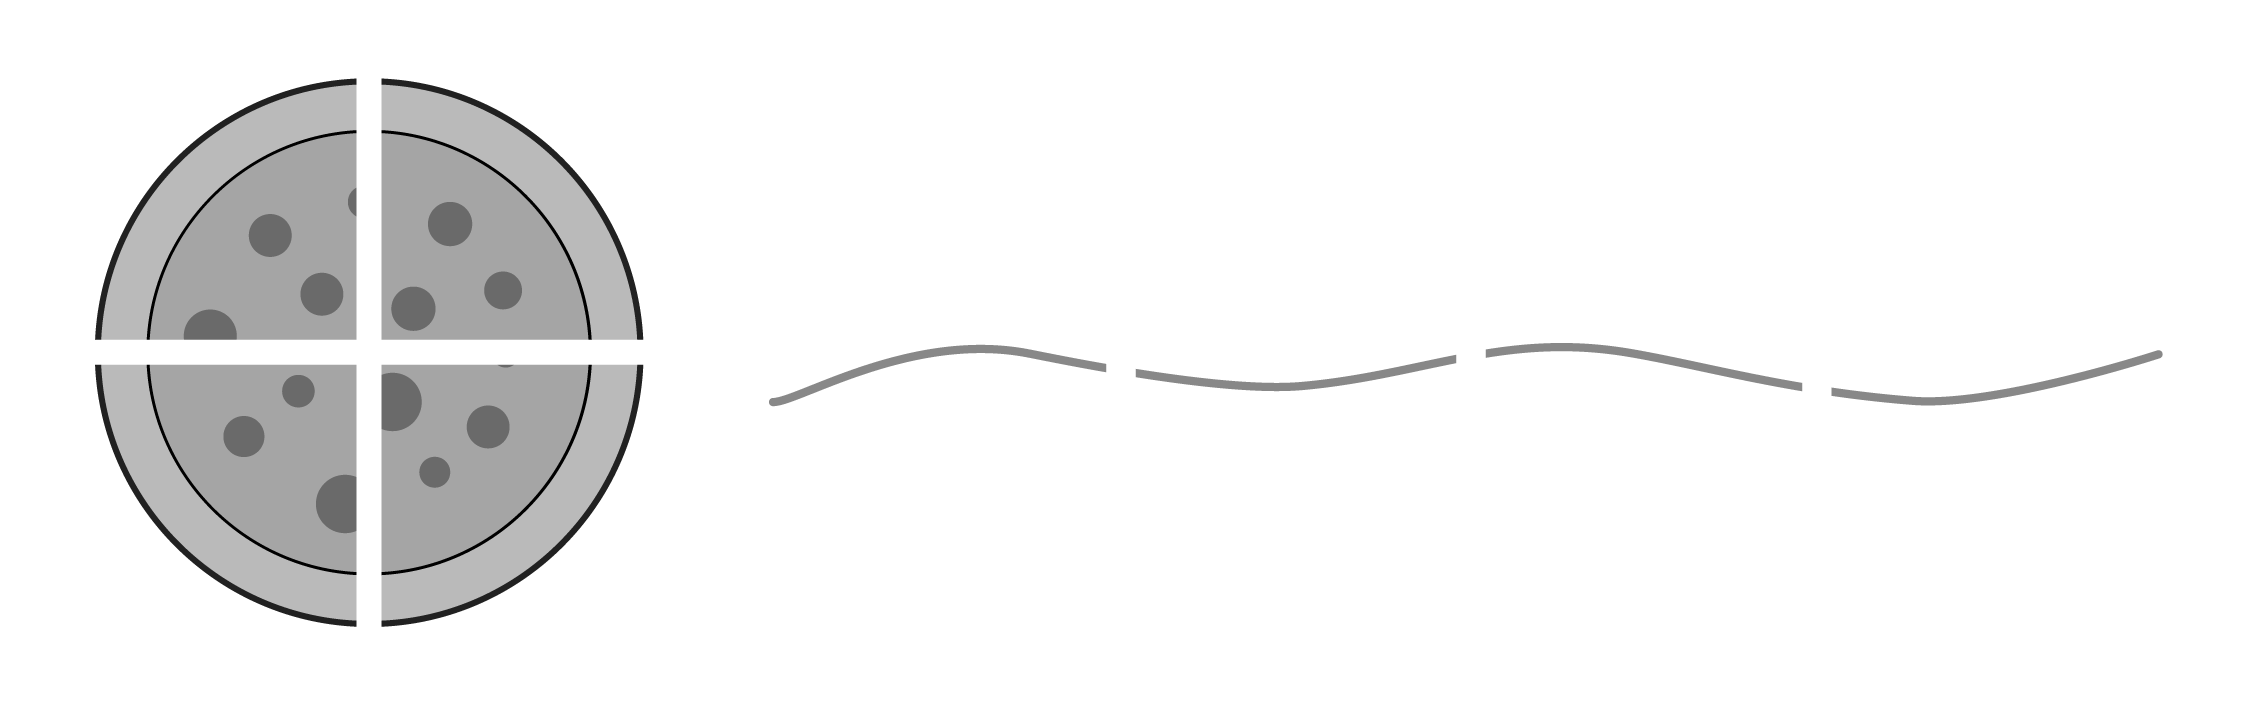
\includegraphics[width=.9\textwidth, keepaspectratio]{licao02/orgideias_fig01.png}
  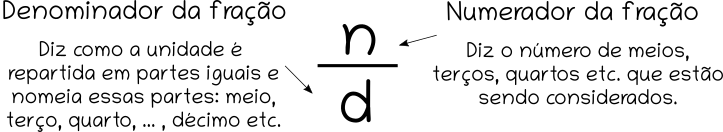
\includegraphics[width=.9\textwidth, keepaspectratio]{licao02/orgideias_fig01b.png}
\end{center}

\begin{itemize}
\item Em $\frac{2}{5}$, por exemplo, o numerador é 2 e o denominador é 5. Lê-se \textit{{dois quintos}}.
\item Em $\frac{10}{8}$, por exemplo, o numerador é 10 e o denominador é 8. Lê-se \textit{{ dez oitavos}}.
\end{itemize}


Para ler a fração deve-se ler o {\bfseries número} do numerador seguido do {\bfseries nome que identifica as partes em que foi repartida a unidade, que é indicado pelo denominador}, nessa ordem. Veja:

\begin{center}
\begin{tabular}[c]{lclcl}
  $\dfrac{1}{3}\rightarrow$ um terço;& \quad & $\dfrac{2}{3}\rightarrow$ dois terços; & \quad & $\dfrac{5}{3}\rightarrow$ cinco terços; \\
  \\
$\dfrac{1}{8}\rightarrow$ um oitavo;& \quad & $\dfrac{3}{8}\rightarrow$ três oitavos; & \quad & $\dfrac{7}{8}\rightarrow$ sete oitavos.  
\end{tabular}
\end{center}

Anote agora os nomes de algumas outras frações:

\begin{center}
  \begin{tabular}[c]{lclcl}
    $\dfrac{1}{2}\rightarrow$  um meio; & \quad & $\dfrac{1}{3}\rightarrow$   um terço; & \quad &  $\dfrac{1}{4}\rightarrow$ um quarto;\\
    \\
    $\dfrac{1}{5}\rightarrow$   um quinto; & \quad &  $\dfrac{1}{6}\rightarrow$  um sexto; & \quad & $\dfrac{1}{7}\rightarrow$  um sétimo;\\
    \\
$\dfrac{1}{8}\rightarrow$   um oitavo; & \quad & $\dfrac{1}{9}\rightarrow$  um nono; & \quad & $\dfrac{1}{10}\rightarrow$   um décimo.
  \end{tabular}
\end{center}

Já a fração $\frac{1}{11}$ não é chamada ``um décimo primeiro''.
Na leitura de frações com denominadores maiores do que 10, utiliza-se a palavra avos.
Assim, a fração $\frac{1}{11}$ é lida ``um onze avos''.
Veja outros exemplos:  
$$\frac{1}{12}\rightarrow \text{  um doze avos;}\quad \frac{1}{13}\rightarrow \text{ um treze avos;} \quad \frac{5}{13}\rightarrow \text{ cinco treze avos.}$$

%Curioso para saber sobre o significado da palavra {\bfseries avos}?
%Pergunte ao seu professor.
%O importante é lembrar que, para denominadores maiores 10, acrescenta-se a expressão ``avos'' ao final da leitura da fração. %Não se esqueça que

Na leitura das frações cujos denominadores são 100, 1000, 1000, etc. não se usa ``avos''. Observe: 
$$\frac{1}{100}\rightarrow \text{ um centésimo;}\quad \frac{13}{100} \rightarrow \text{treze centésimos;} \quad
\frac{33}{1000}\rightarrow \parbox{5em}{trinta e três  milésimos.}$$

{\bfseries Pronto! Agora você já é capaz de ler diversos tipos de frações.}

\section{Mão na Massa}

\begin{atividade}{}\label{chap2-ativ6}
\tikzset{x=1mm,y=1mm}

Uma pizza gigante foi dividida em doze fatias iguais.
Pedro comeu quatro fatias, Isabella cinco fatias, Bernardo duas fatias e Manuela apenas uma fatia.

\begin{center}
  \begin{tabular}{|>{\centering} m{.36\textwidth}|b{0.125\textwidth}|b{0.125\textwidth}|b{0.125\textwidth}|b{0.125\textwidth}|}
\hline
& \centering Pedro & \centering  Isabella & \centering  Bernardo &  \centering Manuela  \tabularnewline
    \hline
   Pinte a fração de pizza consumida  por cada pessoa      & \parbox[c][2cm]{0.125\textwidth}{\centering 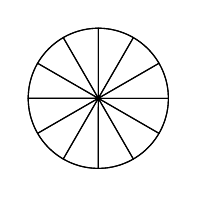
\begin{tikzpicture}[x=1.0cm,y=1.0cm, scale=0.5]
\draw (1.76,2.04) circle (1.78cm);
\draw [shift={(1.76,2.04)}]  (0,0) --  plot[domain=0.:0.5235987755982987,variable=\t]({1.*1.78*cos(\t r)+0.*1.78*sin(\t r)},{0.*1.78*cos(\t r)+1.*1.78*sin(\t r)}) -- cycle ;
\draw [shift={(1.76,2.04)}]  (0,0) --  plot[domain=0.5235987755982987:1.0471975511965974,variable=\t]({1.*1.78*cos(\t r)+0.*1.78*sin(\t r)},{0.*1.78*cos(\t r)+1.*1.78*sin(\t r)}) -- cycle ;
\draw [shift={(1.76,2.04)}]  (0,0) --  plot[domain=1.0471975511965974:1.5707963267948963,variable=\t]({1.*1.78*cos(\t r)+0.*1.78*sin(\t r)},{0.*1.78*cos(\t r)+1.*1.78*sin(\t r)}) -- cycle ;
\draw [shift={(1.76,2.04)}]  (0,0) --  plot[domain=1.5707963267948963:2.0943951023931953,variable=\t]({1.*1.78*cos(\t r)+0.*1.78*sin(\t r)},{0.*1.78*cos(\t r)+1.*1.78*sin(\t r)}) -- cycle ;
\draw [shift={(1.76,2.04)}]  (0,0) --  plot[domain=2.0943951023931953:2.617993877991494,variable=\t]({1.*1.78*cos(\t r)+0.*1.78*sin(\t r)},{0.*1.78*cos(\t r)+1.*1.78*sin(\t r)}) -- cycle ;
\draw [shift={(1.76,2.04)}]  (0,0) --  plot[domain=2.617993877991494:3.1415926535897927,variable=\t]({1.*1.78*cos(\t r)+0.*1.78*sin(\t r)},{0.*1.78*cos(\t r)+1.*1.78*sin(\t r)}) -- cycle ;
\draw [shift={(1.76,2.04)}]  (0,0) --  plot[domain=3.1415926535897927:3.6651914291880914,variable=\t]({1.*1.78*cos(\t r)+0.*1.78*sin(\t r)},{0.*1.78*cos(\t r)+1.*1.78*sin(\t r)}) -- cycle ;
\draw [shift={(1.76,2.04)}]  (0,0) --  plot[domain=3.6651914291880914:4.18879020478639,variable=\t]({1.*1.78*cos(\t r)+0.*1.78*sin(\t r)},{0.*1.78*cos(\t r)+1.*1.78*sin(\t r)}) -- cycle ;
\draw [shift={(1.76,2.04)}]  (0,0) --  plot[domain=4.18879020478639:4.712388980384689,variable=\t]({1.*1.78*cos(\t r)+0.*1.78*sin(\t r)},{0.*1.78*cos(\t r)+1.*1.78*sin(\t r)}) -- cycle ;
\draw [shift={(1.76,2.04)}]  (0,0) --  plot[domain=4.712388980384689:5.235987755982988,variable=\t]({1.*1.78*cos(\t r)+0.*1.78*sin(\t r)},{0.*1.78*cos(\t r)+1.*1.78*sin(\t r)}) -- cycle ;
\draw [shift={(1.76,2.04)}]  (0,0) --  plot[domain=5.235987755982988:5.759586531581286,variable=\t]({1.*1.78*cos(\t r)+0.*1.78*sin(\t r)},{0.*1.78*cos(\t r)+1.*1.78*sin(\t r)}) -- cycle ;
\draw [shift={(1.76,2.04)}]  (0,0) --  plot[domain=-0.5235987755983:0.,variable=\t]({1.*1.78*cos(\t r)+0.*1.78*sin(\t r)},{0.*1.78*cos(\t r)+1.*1.78*sin(\t r)}) -- cycle ;
\end{tikzpicture}}
  & \parbox[c][2cm]{0.125\textwidth}{\centering 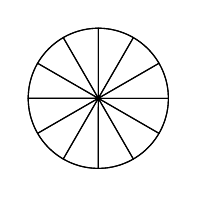
\begin{tikzpicture}[x=1.0cm,y=1.0cm, scale=0.5]
\draw (1.76,2.04) circle (1.78cm);
\draw [shift={(1.76,2.04)}]  (0,0) --  plot[domain=0.:0.5235987755982987,variable=\t]({1.*1.78*cos(\t r)+0.*1.78*sin(\t r)},{0.*1.78*cos(\t r)+1.*1.78*sin(\t r)}) -- cycle ;
\draw [shift={(1.76,2.04)}]  (0,0) --  plot[domain=0.5235987755982987:1.0471975511965974,variable=\t]({1.*1.78*cos(\t r)+0.*1.78*sin(\t r)},{0.*1.78*cos(\t r)+1.*1.78*sin(\t r)}) -- cycle ;
\draw [shift={(1.76,2.04)}]  (0,0) --  plot[domain=1.0471975511965974:1.5707963267948963,variable=\t]({1.*1.78*cos(\t r)+0.*1.78*sin(\t r)},{0.*1.78*cos(\t r)+1.*1.78*sin(\t r)}) -- cycle ;
\draw [shift={(1.76,2.04)}]  (0,0) --  plot[domain=1.5707963267948963:2.0943951023931953,variable=\t]({1.*1.78*cos(\t r)+0.*1.78*sin(\t r)},{0.*1.78*cos(\t r)+1.*1.78*sin(\t r)}) -- cycle ;
\draw [shift={(1.76,2.04)}]  (0,0) --  plot[domain=2.0943951023931953:2.617993877991494,variable=\t]({1.*1.78*cos(\t r)+0.*1.78*sin(\t r)},{0.*1.78*cos(\t r)+1.*1.78*sin(\t r)}) -- cycle ;
\draw [shift={(1.76,2.04)}]  (0,0) --  plot[domain=2.617993877991494:3.1415926535897927,variable=\t]({1.*1.78*cos(\t r)+0.*1.78*sin(\t r)},{0.*1.78*cos(\t r)+1.*1.78*sin(\t r)}) -- cycle ;
\draw [shift={(1.76,2.04)}]  (0,0) --  plot[domain=3.1415926535897927:3.6651914291880914,variable=\t]({1.*1.78*cos(\t r)+0.*1.78*sin(\t r)},{0.*1.78*cos(\t r)+1.*1.78*sin(\t r)}) -- cycle ;
\draw [shift={(1.76,2.04)}]  (0,0) --  plot[domain=3.6651914291880914:4.18879020478639,variable=\t]({1.*1.78*cos(\t r)+0.*1.78*sin(\t r)},{0.*1.78*cos(\t r)+1.*1.78*sin(\t r)}) -- cycle ;
\draw [shift={(1.76,2.04)}]  (0,0) --  plot[domain=4.18879020478639:4.712388980384689,variable=\t]({1.*1.78*cos(\t r)+0.*1.78*sin(\t r)},{0.*1.78*cos(\t r)+1.*1.78*sin(\t r)}) -- cycle ;
\draw [shift={(1.76,2.04)}]  (0,0) --  plot[domain=4.712388980384689:5.235987755982988,variable=\t]({1.*1.78*cos(\t r)+0.*1.78*sin(\t r)},{0.*1.78*cos(\t r)+1.*1.78*sin(\t r)}) -- cycle ;
\draw [shift={(1.76,2.04)}]  (0,0) --  plot[domain=5.235987755982988:5.759586531581286,variable=\t]({1.*1.78*cos(\t r)+0.*1.78*sin(\t r)},{0.*1.78*cos(\t r)+1.*1.78*sin(\t r)}) -- cycle ;
\draw [shift={(1.76,2.04)}]  (0,0) --  plot[domain=-0.5235987755983:0.,variable=\t]({1.*1.78*cos(\t r)+0.*1.78*sin(\t r)},{0.*1.78*cos(\t r)+1.*1.78*sin(\t r)}) -- cycle ;
\end{tikzpicture}}
   & \parbox[c][2cm]{0.125\textwidth}{\centering 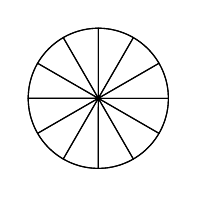
\begin{tikzpicture}[x=1.0cm,y=1.0cm, scale=0.5]
\draw (1.76,2.04) circle (1.78cm);
\draw [shift={(1.76,2.04)}]  (0,0) --  plot[domain=0.:0.5235987755982987,variable=\t]({1.*1.78*cos(\t r)+0.*1.78*sin(\t r)},{0.*1.78*cos(\t r)+1.*1.78*sin(\t r)}) -- cycle ;
\draw [shift={(1.76,2.04)}]  (0,0) --  plot[domain=0.5235987755982987:1.0471975511965974,variable=\t]({1.*1.78*cos(\t r)+0.*1.78*sin(\t r)},{0.*1.78*cos(\t r)+1.*1.78*sin(\t r)}) -- cycle ;
\draw [shift={(1.76,2.04)}]  (0,0) --  plot[domain=1.0471975511965974:1.5707963267948963,variable=\t]({1.*1.78*cos(\t r)+0.*1.78*sin(\t r)},{0.*1.78*cos(\t r)+1.*1.78*sin(\t r)}) -- cycle ;
\draw [shift={(1.76,2.04)}]  (0,0) --  plot[domain=1.5707963267948963:2.0943951023931953,variable=\t]({1.*1.78*cos(\t r)+0.*1.78*sin(\t r)},{0.*1.78*cos(\t r)+1.*1.78*sin(\t r)}) -- cycle ;
\draw [shift={(1.76,2.04)}]  (0,0) --  plot[domain=2.0943951023931953:2.617993877991494,variable=\t]({1.*1.78*cos(\t r)+0.*1.78*sin(\t r)},{0.*1.78*cos(\t r)+1.*1.78*sin(\t r)}) -- cycle ;
\draw [shift={(1.76,2.04)}]  (0,0) --  plot[domain=2.617993877991494:3.1415926535897927,variable=\t]({1.*1.78*cos(\t r)+0.*1.78*sin(\t r)},{0.*1.78*cos(\t r)+1.*1.78*sin(\t r)}) -- cycle ;
\draw [shift={(1.76,2.04)}]  (0,0) --  plot[domain=3.1415926535897927:3.6651914291880914,variable=\t]({1.*1.78*cos(\t r)+0.*1.78*sin(\t r)},{0.*1.78*cos(\t r)+1.*1.78*sin(\t r)}) -- cycle ;
\draw [shift={(1.76,2.04)}]  (0,0) --  plot[domain=3.6651914291880914:4.18879020478639,variable=\t]({1.*1.78*cos(\t r)+0.*1.78*sin(\t r)},{0.*1.78*cos(\t r)+1.*1.78*sin(\t r)}) -- cycle ;
\draw [shift={(1.76,2.04)}]  (0,0) --  plot[domain=4.18879020478639:4.712388980384689,variable=\t]({1.*1.78*cos(\t r)+0.*1.78*sin(\t r)},{0.*1.78*cos(\t r)+1.*1.78*sin(\t r)}) -- cycle ;
\draw [shift={(1.76,2.04)}]  (0,0) --  plot[domain=4.712388980384689:5.235987755982988,variable=\t]({1.*1.78*cos(\t r)+0.*1.78*sin(\t r)},{0.*1.78*cos(\t r)+1.*1.78*sin(\t r)}) -- cycle ;
\draw [shift={(1.76,2.04)}]  (0,0) --  plot[domain=5.235987755982988:5.759586531581286,variable=\t]({1.*1.78*cos(\t r)+0.*1.78*sin(\t r)},{0.*1.78*cos(\t r)+1.*1.78*sin(\t r)}) -- cycle ;
\draw [shift={(1.76,2.04)}]  (0,0) --  plot[domain=-0.5235987755983:0.,variable=\t]({1.*1.78*cos(\t r)+0.*1.78*sin(\t r)},{0.*1.78*cos(\t r)+1.*1.78*sin(\t r)}) -- cycle ;
\end{tikzpicture}}
  & \parbox[c][2cm]{0.125\textwidth}{\centering 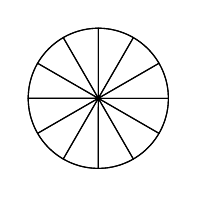
\begin{tikzpicture}[x=1.0cm,y=1.0cm, scale=0.5]
\draw (1.76,2.04) circle (1.78cm);
\draw [shift={(1.76,2.04)}]  (0,0) --  plot[domain=0.:0.5235987755982987,variable=\t]({1.*1.78*cos(\t r)+0.*1.78*sin(\t r)},{0.*1.78*cos(\t r)+1.*1.78*sin(\t r)}) -- cycle ;
\draw [shift={(1.76,2.04)}]  (0,0) --  plot[domain=0.5235987755982987:1.0471975511965974,variable=\t]({1.*1.78*cos(\t r)+0.*1.78*sin(\t r)},{0.*1.78*cos(\t r)+1.*1.78*sin(\t r)}) -- cycle ;
\draw [shift={(1.76,2.04)}]  (0,0) --  plot[domain=1.0471975511965974:1.5707963267948963,variable=\t]({1.*1.78*cos(\t r)+0.*1.78*sin(\t r)},{0.*1.78*cos(\t r)+1.*1.78*sin(\t r)}) -- cycle ;
\draw [shift={(1.76,2.04)}]  (0,0) --  plot[domain=1.5707963267948963:2.0943951023931953,variable=\t]({1.*1.78*cos(\t r)+0.*1.78*sin(\t r)},{0.*1.78*cos(\t r)+1.*1.78*sin(\t r)}) -- cycle ;
\draw [shift={(1.76,2.04)}]  (0,0) --  plot[domain=2.0943951023931953:2.617993877991494,variable=\t]({1.*1.78*cos(\t r)+0.*1.78*sin(\t r)},{0.*1.78*cos(\t r)+1.*1.78*sin(\t r)}) -- cycle ;
\draw [shift={(1.76,2.04)}]  (0,0) --  plot[domain=2.617993877991494:3.1415926535897927,variable=\t]({1.*1.78*cos(\t r)+0.*1.78*sin(\t r)},{0.*1.78*cos(\t r)+1.*1.78*sin(\t r)}) -- cycle ;
\draw [shift={(1.76,2.04)}]  (0,0) --  plot[domain=3.1415926535897927:3.6651914291880914,variable=\t]({1.*1.78*cos(\t r)+0.*1.78*sin(\t r)},{0.*1.78*cos(\t r)+1.*1.78*sin(\t r)}) -- cycle ;
\draw [shift={(1.76,2.04)}]  (0,0) --  plot[domain=3.6651914291880914:4.18879020478639,variable=\t]({1.*1.78*cos(\t r)+0.*1.78*sin(\t r)},{0.*1.78*cos(\t r)+1.*1.78*sin(\t r)}) -- cycle ;
\draw [shift={(1.76,2.04)}]  (0,0) --  plot[domain=4.18879020478639:4.712388980384689,variable=\t]({1.*1.78*cos(\t r)+0.*1.78*sin(\t r)},{0.*1.78*cos(\t r)+1.*1.78*sin(\t r)}) -- cycle ;
\draw [shift={(1.76,2.04)}]  (0,0) --  plot[domain=4.712388980384689:5.235987755982988,variable=\t]({1.*1.78*cos(\t r)+0.*1.78*sin(\t r)},{0.*1.78*cos(\t r)+1.*1.78*sin(\t r)}) -- cycle ;
\draw [shift={(1.76,2.04)}]  (0,0) --  plot[domain=5.235987755982988:5.759586531581286,variable=\t]({1.*1.78*cos(\t r)+0.*1.78*sin(\t r)},{0.*1.78*cos(\t r)+1.*1.78*sin(\t r)}) -- cycle ;
\draw [shift={(1.76,2.04)}]  (0,0) --  plot[domain=-0.5235987755983:0.,variable=\t]({1.*1.78*cos(\t r)+0.*1.78*sin(\t r)},{0.*1.78*cos(\t r)+1.*1.78*sin(\t r)}) -- cycle ;
\end{tikzpicture}}
  \\
    \hline
     Escreva, por extenso, a fra\-ção de pizza consumida por cada pessoa&                                        &                                        &                                         &                                        \\
    \hline
     Escreva, usando símbolos ma\-temáticos, a fração de pizza consumida por cada pessoa &                                        &                                        &                                         &                                        \\
    \hline
  \end{tabular}
\end{center}

\begin{enumerate}  %d
  \item Na sua opinião, qual maneira de representar fração ``gasta menos lápis'': pintando, escrevendo por extenso ou usando símbolos matemáticos?
  \item Na sua opinião, qual a representação que mais rapidamente ajuda a decidir quem comeu mais e quem comeu menos pizza?
\end{enumerate} %d
\end{atividade}

\begin{atividade}{}\label{chap2-ativ7}
Um grupo de amigos está dividindo duas pizzas circulares iguais, isto é, de mesmo tamanho. A primeira pizza foi cortada em 4 fatias de mesmo tamanho. A segunda pizza foi repartida em 8 pedaços iguais.
\begin{enumerate}  %s
\item Uma fatia da primeira pizza é que fração dessa pizza? Responda usando símbolos matemáticos.
\item Uma fatia da segunda pizza é que fração dessa pizza? Responda usando símbolos matemáticos.
\item Qual fatia tem mais quantidade de pizza: uma fatia da primeira ou uma fatia da segunda? Explique usando uma figura.
\end{enumerate} %s
\end{atividade}

\begin{atividade}{}\label{chap2-ativ8}
Para cada figura a seguir, indique a fração da figura que está em destaque. Esta fração é maior, menor ou exatamente igual a $\frac{1}{2}$ da figura?


\tikzset{x=1mm,y=1mm}
\begin{enumerate}
\begin{multicols}{3}
\item
\adjustbox{valign=t}
{
\begin{tikzpicture}
\draw[fill=common, fill opacity=.3] (0,0) circle (10);
 \foreach \x in {0,72,...,288}{
 \draw[fill=attention] (0,0) -- (\x:10) arc (\x:\x+36:10) --cycle;
 \draw (\x:10) -- (\x:-10);}
\end{tikzpicture} 
}

\item
\adjustbox{valign=t}
{

\begin{tikzpicture}
\draw[fill=common, fill opacity=.3] (0,0) rectangle (14,20);
\draw[fill=attention] (0,4) rectangle (7,20);
\foreach \y in {4,8,12,16}{
\draw (0,\y)--(14,\y);}
\draw (7,0) -- (7,20);
\end{tikzpicture}
}


\item\adjustbox{valign=t}
{

\begin{tikzpicture}
\draw[fill=common, fill opacity=.3] (0,0) rectangle (30,20);
\fill[attention] (0,0) rectangle (18,20);
 \foreach \x in {3,6,...,27}{
 \draw (\x,0)--(\x,20);}
\end{tikzpicture} 
}

\end{multicols}
\end{enumerate}

\end{atividade}

\clearpage
\begin{atividade}{}\label{chap2-ativ9}

\tikzset{x=1mm,y=1mm}
Na tabela a seguir, pinte cada figura de modo que a parte pintada seja a fração da figura indicada na coluna à esquerda e na mesma linha. Indique também, usando símbolos matemáticos, qual fração da figura ficou sem ser pintada.

\begin{center}
\
 \scalebox{.95}{\begin{tabular}{|m{0.33\textwidth}|c|m{0.33\textwidth}|}
     \hline
       \centering Fração da figura que deve ser pintada  & \parbox[c]{1.6cm}{\centering Figura}  & \centering   Fração da figura que ficou sem ser pintada  \tabularnewline
     \hline
      \centering $\dfrac{5}{6}$  & \centering \parbox[c][2cm][c]{1.6cm}{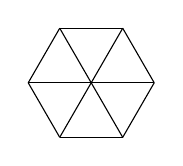
\begin{tikzpicture}
                                     \foreach \x in {0,60,...,300}{ \draw (0,0)--(\x:8);\draw (\x:8)--(\x+60:8);}
                                    \end{tikzpicture}}
 &  \\
     \hline
      \centering $\dfrac{3}{4}$  &  \centering \parbox[c][2cm][c]{1.6cm}{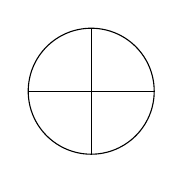
\begin{tikzpicture}
                                     \draw (0:8)--(180:8);
                                     \draw (90:8)--(270:8);
                                     \draw (0,0) circle (8);
                                    \end{tikzpicture}}
                                    &  \\
     \hline
      \centering $\dfrac{2}{5}$  &   \centering \parbox[c][2cm][c]{2.5cm}{
                                     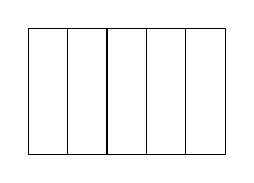
\begin{tikzpicture}
                                     \draw (0,0) rectangle (25,16);
                                     \foreach \x in {5,10,15,20}{\draw (\x,0)--(\x,16);}
                                    \end{tikzpicture} }
                                    &  \\
     \hline
      \centering $\dfrac{2}{3}$  &  \centering \parbox[c][2cm][c]{1.6cm}{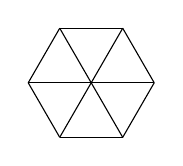
\begin{tikzpicture}
                                     \foreach \x in {0,60,...,300}{ \draw (0,0)--(\x:8);\draw (\x:8)--(\x+60:8);}
                                    \end{tikzpicture}}
                                    &  \\
     \hline
      \centering $\dfrac{3}{8}$  &   \centering \parbox[c][2cm][c]{1.6cm}{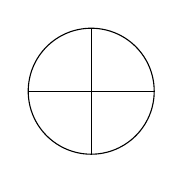
\begin{tikzpicture}
                                     \draw (0:8)--(180:8);
                                     \draw (90:8)--(270:8);
                                     \draw (0,0) circle (8);
                                    \end{tikzpicture}}&  \\
     \hline
      \centering $\dfrac{9}{10}$  & \centering \parbox[c][2cm][c]{2.5cm}{
                                     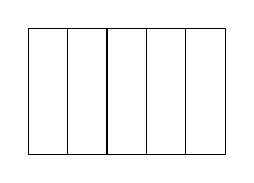
\begin{tikzpicture}
                                     \draw (0,0) rectangle (25,16);
                                     \foreach \x in {5,10,15,20}{\draw (\x,0)--(\x,16);}
                                    \end{tikzpicture} }
                                    &  \\
     \hline
   \end{tabular}}
\end{center}
\end{atividade}

\begin{atividade}{}\label{chap2-ativ10}
A figura mostra três copos idênticos.  É possível armazenar a água dos três copos em um único copo sem que transborde? Explique usando frações.

% \begin{center}
% \begin{tikzpicture}[scale=0.3, x=1cm,y=1cm]

% % Definição do eixo vertical das elipses
% \def\EixoM{0.5}

% % colorindo o primeiro cilindro
% \fill[common] (2,0) ellipse (2 and \EixoM);
% \fill[common] (0,0) rectangle (4,3);
% \fill[common] (2,3) ellipse (2 and \EixoM);

% % colorindo o segundo cilindro
% \fill[common] (8,0) ellipse (2 and \EixoM);
% \fill[common] (6,0) rectangle (10,2);
% \fill[common] (8,2) ellipse (2 and \EixoM);

% % colorindo o terceiro
% \fill[common] (14,0) ellipse (2 and \EixoM);
% \fill[common] (12,0) rectangle (16,4);
% \fill[common] (14,4) ellipse (2 and \EixoM);

% % shift horizontal nos cilindros definido por \x
% \foreach \x in {0,6,12}{
% \draw (\x,0)--(\x,8);
% \draw (\x + 4,0)--(\x + 4,8);
% % shift vertical nos arcos de elipse definido por \y
% \foreach \y in {0,1,...,7}{
% \pgfpathmoveto{\pgfpoint{\x cm}{\y cm}}
% \pgfpatharc{-180}{0}{2cm and \EixoM cm}
% \pgfusepath{draw}}
% \draw (\x + 2,8) ellipse (2 and \EixoM);}

% \node at (2,-2) {(1)};
% \node at (8,-2) {(2)};
% \node at (14,-2) {(3)};
% \end{tikzpicture}

% \end{center}

\begin{figure}[H]
\centering

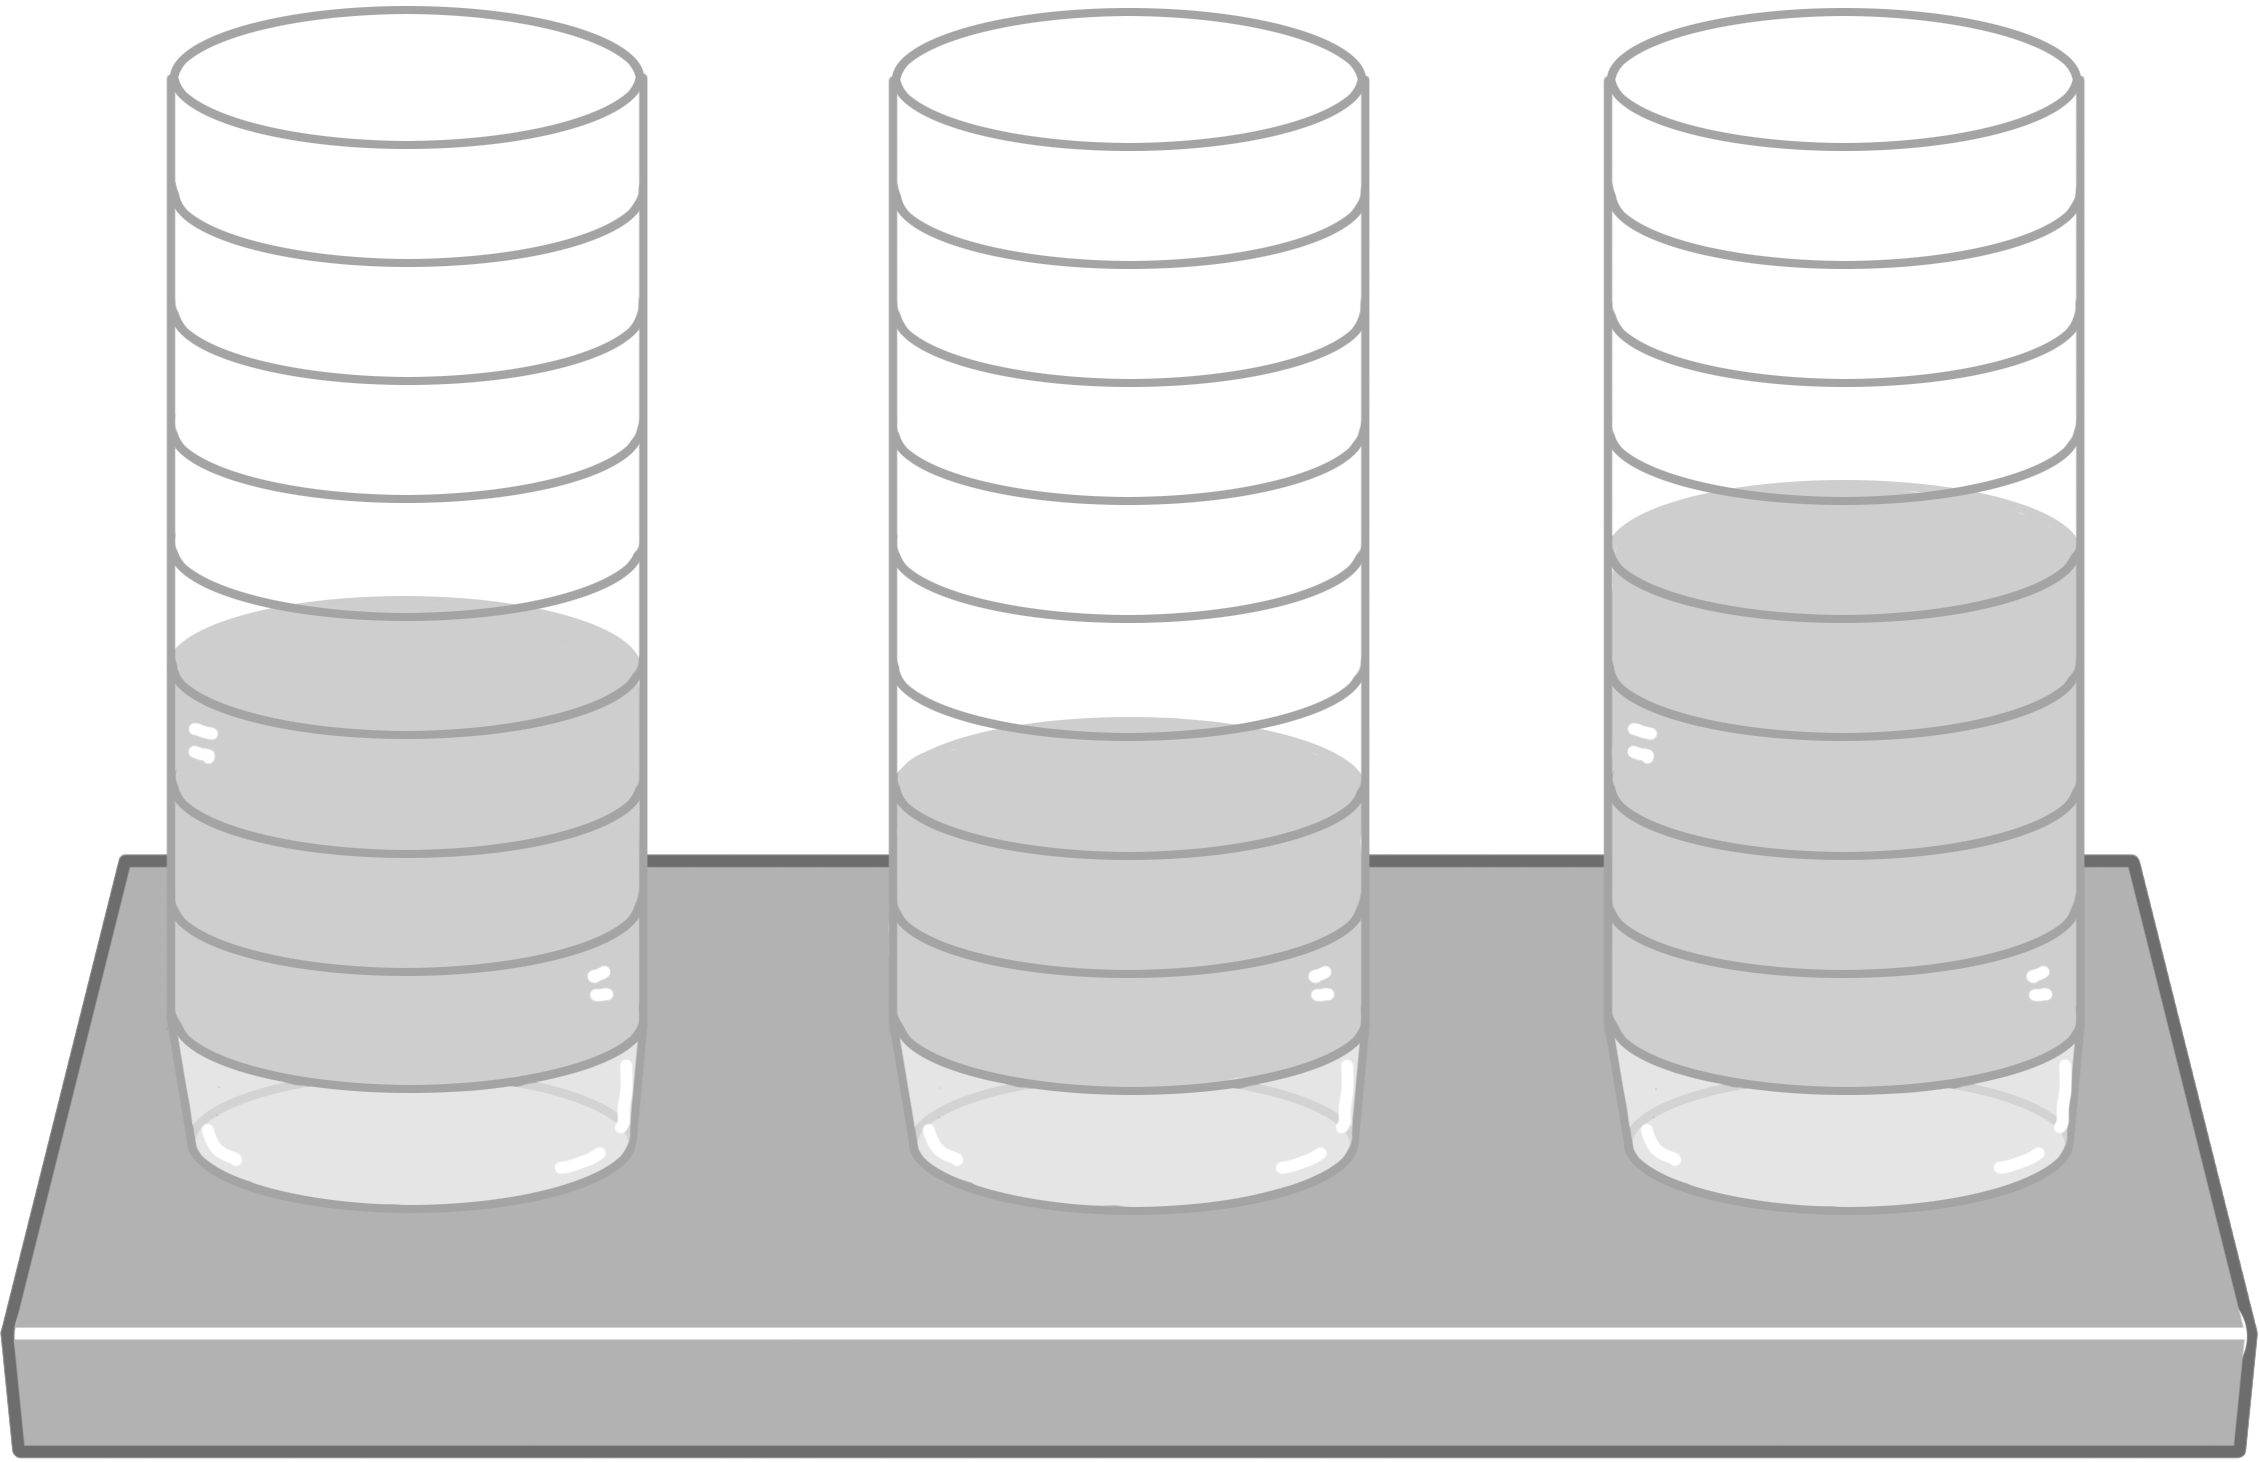
\includegraphics[width=.4\linewidth]{licao02/ativ10-fig01}
\end{figure}
\end{atividade}

\begin{atividade}
\tikzset{x=1mm,y=1mm}
\newcommand\fit[1]{\parbox[c][1.35cm]{.2\textwidth}{\centering#1}}
\begin{center}
  \begin{tabular}{|m{0.2\textwidth}|m{0.3\textwidth}|c|}
    \hline
     \centering Fração da unidade  & \centering  Figura correspondente à fração da unidade  & \centering Desenhe aqui a unidade  \tabularnewline
    \hline 
     \centering \fit{$\dfrac{1}{2}$}  &\centering \parbox[c][1.35cm]{1.5cm}{\centering\begin{tikzpicture}
                                    \draw[fill=common, fill opacity=.3] (0,0) rectangle (12,6);
                                   \end{tikzpicture}}
 &  \\
    \hline
     \centering \fit{$\dfrac{4}{2}$}  &   \centering \parbox[c][1.35cm]{1.5cm}{\centering\begin{tikzpicture}
                                    \draw[fill=common, fill opacity=.3] (0,0) rectangle (12,6);
                                   \end{tikzpicture}}
                                   &  \\
    \hline
     \centering \fit{$\dfrac{3}{2}$}  &  \centering \parbox[c][1.35cm]{1.5cm}{\centering\begin{tikzpicture}
                                    \draw[fill=common, fill opacity=.3] (0,0) rectangle (12,6);
                                   \end{tikzpicture}}
                                   &  \\
    \hline
     \centering \fit{$\dfrac{2}{3}$}  &  \centering \parbox[c][1.35cm]{1.5cm}{\centering\begin{tikzpicture}
                                    \draw[fill=common, fill opacity=.3] (0,0) rectangle (12,6);
                                   \end{tikzpicture}}
                                   &  \\
    \hline
     \centering \fit{$\dfrac{1}{2}$}  &  \centering \parbox[c][1.35cm]{1.5cm}{\centering\begin{tikzpicture}
                                    \draw[fill=common, fill opacity=.3] (0,0) arc (0:180:6) -- cycle;
                                   \end{tikzpicture}}  &  \\
    \hline
      \centering \fit{$\dfrac{4}{2}$}  &  \centering \parbox[c][1.35cm]{1.5cm}{\centering\begin{tikzpicture}
                                    \draw[fill=common, fill opacity=.3] (0,0) arc (0:180:6) -- cycle;
                                   \end{tikzpicture}} &  \\
    \hline
      \centering \fit{$\dfrac{3}{2}$}  &  \centering \parbox[c][1.35cm]{1.5cm}{\centering\begin{tikzpicture}
                                    \draw[fill=common, fill opacity=.3] (0,0) arc (0:180:6) -- cycle;
                                   \end{tikzpicture}}  &  \\
    \hline
      \centering \fit{$\dfrac{2}{3}$}  &  \centering \parbox[c][1.35cm]{1.5cm}{\centering\begin{tikzpicture}
                                    \draw[fill=common, fill opacity=.3] (0,0) arc (0:180:6) -- cycle;
                                   \end{tikzpicture}} &  \\
    \hline
      \centering \fit{$\dfrac{1}{2}$}  &  \centering \parbox[c][1.35cm]{1.5cm}{\centering\begin{tikzpicture}
                                    \draw[fill=common, fill opacity=.3] (0,0) rectangle (12,1);
                                   \end{tikzpicture}}  &  \\
    \hline
      \centering \fit{$\dfrac{4}{2}$}  &  \centering \parbox[c][1.35cm]{1.5cm}{\centering\begin{tikzpicture}
                                    \draw[fill=common, fill opacity=.3] (0,0) rectangle (12,1);
                                   \end{tikzpicture}}  &  \\
    \hline
      \centering \fit{$\dfrac{3}{2}$}  &  \centering \parbox[c][1.35cm]{1.5cm}{\centering\begin{tikzpicture}
                                    \draw[fill=common, fill opacity=.3] (0,0) rectangle (12,1);
                                   \end{tikzpicture}}  &  \\
    \hline
      \centering \fit{$\dfrac{2}{3}$}  &  \centering \parbox[c][1.35cm]{1.5cm}{\centering\begin{tikzpicture}
                                    \draw[fill=common, fill opacity=.3] (0,0) rectangle (12,1);
                                   \end{tikzpicture}}   &  \\
    \hline
        \centering \fit{$\dfrac{1}{2}$}  &  \centering \parbox[c][1.35cm]{1.5cm}{\centering \begin{tikzpicture}
                                      \draw[fill=common, fill opacity=.3] (0:4) -- (60:4)--(120:4)-- (180:4)--(240:4)--(300:4)--cycle;
                                     \end{tikzpicture} } &  \\
     \hline
     \centering \fit{$\dfrac{4}{2}$}  &  \centering \parbox[c][1.35cm]{1.5cm}{\centering \begin{tikzpicture}
                                    \draw[fill=common, fill opacity=.3] (0:4) -- (60:4)--(120:4)-- (180:4)--(240:4)--(300:4)--cycle;
                                   \end{tikzpicture} } &  \\
     \hline
       \centering \fit{$\dfrac{3}{2}$}  &  \centering \parbox[c][1.35cm]{1.5cm}{\centering \begin{tikzpicture}
                                    \draw[fill=common, fill opacity=.3] (0:4) -- (60:4)--(120:4)-- (180:4)--(240:4)--(300:4)--cycle;
                                   \end{tikzpicture} } &  \\
    \hline
      \centering \fit{$\dfrac{2}{3}$}  &  \centering \parbox[c][1.35cm]{1.5cm}{\centering \begin{tikzpicture}
                                    \draw[fill=common, fill opacity=.3] (0:4) -- (60:4)--(120:4)-- (180:4)--(240:4)--(300:4)--cycle;
                                   \end{tikzpicture} } &  \\
    \hline
  \end{tabular}
\end{center}
\end{atividade}



\begin{atividade}{}\label{chap2-ativ11}

Lucas, Matheus, Heitor, Rafael, Enzo, Nicolas, Lorenzo, Guilherme e Samuel estavam brincando de empurrar seus carrinhos de brinquedo para ver qual carrinho ia mais longe em uma pista reta.

A figura a seguir mostra o quão longe foi o carrinho de Lucas e onde ele parou na pista com relação ao ponto de largada.

\begin{figure}[H]
\centering


\includegraphics[width=.85\linewidth]{licao02/pag-25-ativ-12.png}
\end{figure}

Sabe-se que:

\begin{enumerate}[itemsep=.3em, topsep=.5\parskip]  %s
  \item     O carrinho de Matheus só conseguiu ir até a metade da distância percorrida pelo carrinho de Lucas.
  \item     O carrinho de Heitor conseguiu ir até     $\frac{3}{2}$     da distância percorrida pelo carrinho de Lucas.
  \item     O carrinho de Rafael conseguiu ir até     $\frac{4}{2}$     da distância percorrida pelo carrinho de Lucas.
  \item     O carrinho de Enzo conseguiu ir até     $\frac{5}{2}$     da distância percorrida pelo carrinho de Lucas.
  \item     O carrinho de Nicolas conseguiu ir até     $\frac{6}{2}$     da distância percorrida pelo carrinho de Lucas.
  \item     O carrinho de Lorenzo conseguiu ir até     $\frac{6}{4}$     da distância percorrida pelo carrinho de Lucas.
  \item     O carrinho de Guilherme conseguiu ir até o dobro da distância percorrida pelo carrinho de Lucas.
  \item     O carrinho de Samuel conseguiu ir até     $\frac{6}{3}$     da distância percorrida pelo carrinho de Lucas.
\end{enumerate} %s


Com essas informações, marque as posições de parada dos carrinhos de todos os amigos de Lucas no encarte que você irá receber.

\begin{figure}[H]
\centering

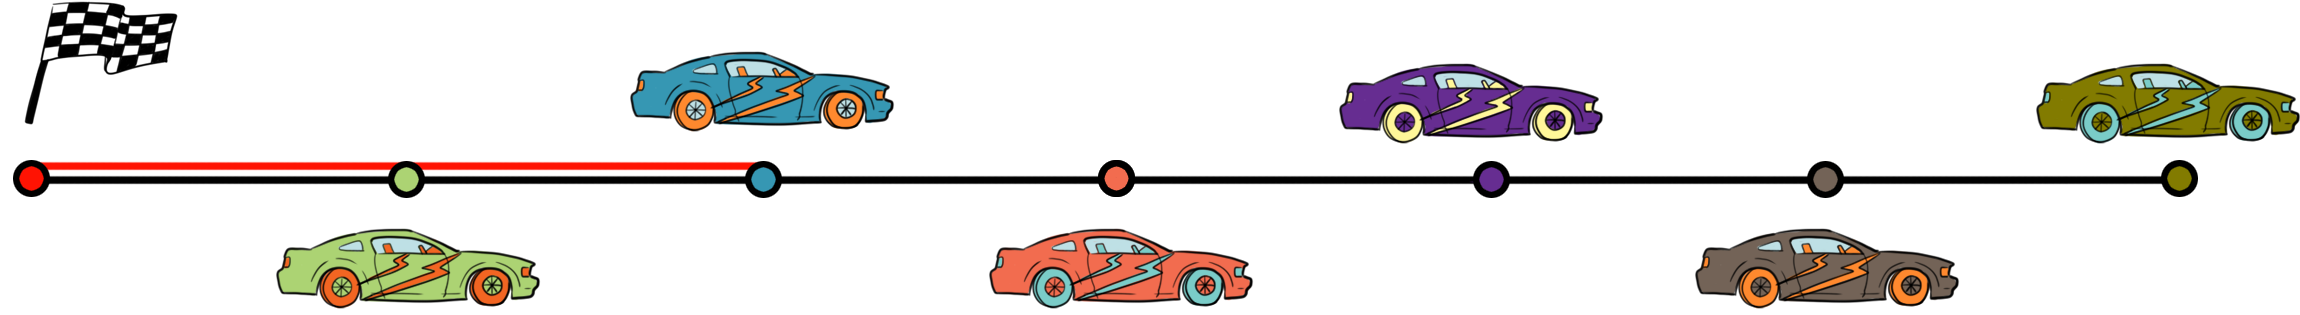
\includegraphics[width=.85\linewidth]{licao02/pag-26-ativ-12.png}
\end{figure}


Os carrinhos de Rafael e Samuel pararam no mesmo lugar? Explique.
\end{atividade}

\begin{atividade}{}\label{chap2-ativ12}

Anita, Gustavo e Henrique descobriram que todos tinham levado bolo para o lanche.\newline
Anita falou: ``Mamãe colocou metade do bolo no meu lanche.''\newline
Gustavo falou: ``Eu trouxe um terço do bolo que minha tia fez.''\newline
Henrique falou: ``Eu trouxe apenas um quinto do bolo que minha mãe preparou!''\newline
Para surpresa de todos, ao retirarem seus lanches da mochila, descobriram que todos traziam-no em  embalagens iguais, portanto traziam a mesma \linebreak quantidade de bolo.\newline
Como você explica tal situação?
\end{atividade}

\section{Quebrando a Cuca}


\begin{atividade}{}\label{chap2-ativ13}

(NAEP, 1992) Pense cuidadosamente nesta questão. Escreva uma resposta completa. Você pode usar desenhos, palavras e números para explicar sua resposta. Certifique-se de mostrar todo o seu raciocínio.

José comeu $\frac{1}{2}$ de uma pizza. Ella comeu $\frac{1}{2}$ de uma outra pizza. José disse que ele comeu mais pizza do que Ella, mas Ella diz que eles comeram a mesma quantidade. Use palavras, figuras ou números para mostrar que José pode estar certo.
\end{atividade}

\clearpage
\begin{atividade}{}\label{chap2-ativ14}
\tikzset{x=1mm,y=1mm}

Complete as sentenças a seguir com uma fração adequada (usando símbolos matemáticos). Perceba que uma mesma região pintada pode ser descrita por frações diferentes, dependendo da unidade considerada.

%definição da região limitada pelos 2 hexágonos encaixados.
\def \tripinha{ (30:4) -- (90:4) -- (150:4)--(210:4)--(270:4)--(330:4) [shift={({4*sqrt(3)},0)}] --(270:4) -- (330:4) -- (30:4) -- (90:4)--(150:4)--cycle;}
%definição da região limitada pelos 3 hexágonos encaixados.
\def \tripa{ (30:4) -- (90:4) -- (150:4)--(210:4)--(270:4)--(330:4) [shift={({4*sqrt(3)},0)}] --(270:4) -- (330:4) [shift={({4*sqrt(3)},0)}]--  (270:4) -- (330:4) -- (30:4) -- (90:4)--(150:4) [shift={({-4*sqrt(3)},0)}] -- (90:4) -- (150:4)--cycle;}

\begin{enumerate}  %s
%a
\item     A região em destaque na figura
\begin{tikzpicture}[scale=1.3]
 \draw \tripa;
\begin{scope}
 \clip \tripa;
\draw[fill=attention] (-4,-4) rectangle (0,4);
\draw[fill=common, fill opacity=.3] (0,-4) rectangle (20,4);
\end{scope}
\end{tikzpicture} 
é \hrulefill de 
\begin{tikzpicture}[scale=1.3]
\draw[fill=common, fill opacity=.3] (30:4) -- (90:4) -- (150:4) -- (210:4) -- (270:4) -- (330:4)--cycle;
\end{tikzpicture}.
 %b
\item     A região em destaque na figura
\begin{tikzpicture}[scale=1.3]
 \draw \tripa;
\begin{scope}
 \clip \tripa;
\draw[fill=attention] (-4,-4) rectangle (0,4);
\draw[fill=common, fill opacity=.3] (0,-4) rectangle (20,4);
\end{scope}
\end{tikzpicture}
é
\hrulefill
de
\begin{tikzpicture}[scale=1.3]
 \draw[fill=common, fill opacity=.3] (30:4) -- (90:4) -- (150:4)--(210:4)--(270:4)--(330:4) [shift={({4*sqrt(3)},0)}] --(270:4) -- (330:4) --(30:4) -- (90:4) -- (150:4)--cycle;
\end{tikzpicture}.

%c
\item     A região em destaque na figura \begin{tikzpicture}[scale=1.3]
 \draw \tripa;
\begin{scope}
 \clip \tripa;
\draw[fill=attention] (-4,-4) rectangle (0,4);
\draw[fill=common, fill opacity=.3] (0,-4) rectangle (20,4);
\end{scope}
\end{tikzpicture}
     é \hrulefill    de
\begin{tikzpicture}[scale=1.3]
\draw[fill=common, fill opacity=.3] \tripa;
\end{tikzpicture}.

%d
 \item     A região em destaque na figura  \begin{tikzpicture}[scale=1.3]
 \draw \tripa;
\begin{scope}
 \clip \tripa;
\draw[fill=attention] (-4,-4) rectangle ({4*sqrt(3)},4);
\draw[fill=common, fill opacity=.3] ({4*sqrt(3)},-4) rectangle ({10*sqrt(3)},4);
\end{scope}
\end{tikzpicture}  é \hrulefill    de
\begin{tikzpicture}[scale=1.3]
\draw[fill=common, fill opacity=.3] (30:4) -- (90:4) -- (150:4) -- (210:4) -- (270:4) -- (330:4)--cycle;
\end{tikzpicture}.
%e
\item     A região em destaque na figura   \begin{tikzpicture}[scale=1.3]
 \draw \tripa;
\begin{scope}
 \clip \tripa;
\draw[fill=attention] (-4,-4) rectangle ({4*sqrt(3)},4);
\draw[fill=common, fill opacity=.3] ({4*sqrt(3)},-4) rectangle ({10*sqrt(3)},4);
\end{scope}
\end{tikzpicture}    é \hrulefill    de
\begin{tikzpicture}[scale=1.3]
 \draw[fill=common, fill opacity=.3] (30:4) -- (90:4) -- (150:4)--(210:4)--(270:4)--(330:4) [shift={({4*sqrt(3)},0)}] --(270:4) -- (330:4) --(30:4) -- (90:4) -- (150:4)--cycle;
\end{tikzpicture}.

%f
\item     A região em destaque na figura  \begin{tikzpicture}[scale=1.3]
 \draw \tripa;
\begin{scope}
 \clip \tripa;
\draw[fill=attention] (-4,-4) rectangle ({4*sqrt(3)},4);
\draw[fill=common, fill opacity=.3] ({4*sqrt(3)},-4) rectangle ({10*sqrt(3)},4);
\end{scope}
\end{tikzpicture}   é \hrulefill    de
\begin{tikzpicture}[scale=1.3]
\draw[fill=common, fill opacity=.3] \tripa;
\end{tikzpicture}.

%g
\item     A região em destaque na figura
\begin{tikzpicture}[scale=1.3]
 \draw \tripa;
\begin{scope}
 \clip \tripa;
\draw[fill=attention] (-4,-4) rectangle ({8*sqrt(3)},4);
\draw[fill=common, fill opacity=.3] ({8*sqrt(3)},-4) rectangle ({10*sqrt(3)},4);
\end{scope}
\end{tikzpicture}
é \hrulefill  de
\begin{tikzpicture}[scale=1.3]
\draw[fill=common, fill opacity=.3] (30:4) -- (90:4) -- (150:4) -- (210:4) -- (270:4) -- (330:4)--cycle;
\end{tikzpicture}.
%h
\item     A região em destaque na figura  \begin{tikzpicture}[scale=1.3]
 \draw \tripa;
\begin{scope}
 \clip \tripa;
\draw[fill=attention] (-4,-4) rectangle ({8*sqrt(3)},4);
\draw[fill=common, fill opacity=.3] ({8*sqrt(3)},-4) rectangle ({10*sqrt(3)},4);
\end{scope}
\end{tikzpicture} é \hrulefill  de
\begin{tikzpicture}[scale=1.3]
 \draw[fill=common, fill opacity=.3] (30:4) -- (90:4) -- (150:4)--(210:4)--(270:4)--(330:4) [shift={({4*sqrt(3)},0)}] --(270:4) -- (330:4) --(30:4) -- (90:4) -- (150:4)--cycle;
\end{tikzpicture}.

%i
\item     A região em destaque na figura
\begin{tikzpicture}[scale=1.3]
 \draw \tripa;
\begin{scope}
 \clip \tripa;
\draw[fill=attention] (-4,-4) rectangle ({8*sqrt(3)},4);
\draw[fill=common, fill opacity=.3] ({8*sqrt(3)},-4) rectangle ({10*sqrt(3)},4);
\end{scope}
\end{tikzpicture}
é \hrulefill    de
\begin{tikzpicture}[scale=1.3]
\draw[fill=common, fill opacity=.3] \tripa;
\end{tikzpicture}.
%j
\item     A região em destaque na figura
  \begin{tikzpicture}[scale=1.3]
 \draw \tripa;
\begin{scope}
 \clip \tripa;
\draw[fill=attention] (-4,-4) rectangle ({12*sqrt(3)},4);
\end{scope}
\end{tikzpicture}
é \hrulefill   de
\begin{tikzpicture}[scale=1.3]
\draw[fill=common, fill opacity=.3] (30:4) -- (90:4) -- (150:4)- - (210:4) -- (270:4) -- (330:4)--cycle;
\end{tikzpicture}.

\setcounter{enumi}{11}
%k
\item     A região em destaque na figura
\begin{tikzpicture}[scale=1.3]
 \draw \tripa;
\begin{scope}
 \clip \tripa;
\draw[fill=attention] (-4,-4) rectangle ({12*sqrt(3)},4);
\end{scope}
\end{tikzpicture}
é \hrulefill de
\begin{tikzpicture}[scale=1.3]
 \draw[fill=common, fill opacity=.3] (30:4) -- (90:4) -- (150:4)--(210:4)--(270:4)--(330:4) [shift={({4*sqrt(3)},0)}] --(270:4) -- (330:4) --(30:4) -- (90:4) -- (150:4)--cycle;
\end{tikzpicture}.

%l
\item     A região em destaque na figura
  \begin{tikzpicture}[scale=1.3]
 \draw \tripa;
\begin{scope}
 \clip \tripa;
\draw[fill=attention] (-4,-4) rectangle ({12*sqrt(3)},4);
\end{scope}
\end{tikzpicture}
é \hrulefill  de
\begin{tikzpicture}[scale=1.3]
\draw[fill=common, fill opacity=.3] \tripa;
\end{tikzpicture}.

\end{enumerate} %s
\end{atividade}

\begin{atividade}{}\label{chap2-ativ15}
\tikzset{x=1mm,y=1mm}

Miguel disse para Alice que a parte em destaque na figura a seguir corresponde a $\frac{3}{5}$ da figura, pois ela está dividida em 5 partes e 3 partes estão pintadas. Você concorda com a afirmação e com a justificativa de Miguel? Explique!

\begin{center}
\begin{tikzpicture}[scale=1.5]
%\fill[fill=attention,fill opacity=0.1] (0.,5.) -- (9.,5.) -- (9.,-5.) -- (0.,-5.) -- cycle;
\filldraw[fill=attention,fill opacity=1.0] (0,0) rectangle (9,5);
\filldraw[fill=common, fill opacity=.3] (0,-5) rectangle (9,0);
%\draw   (0.,5.)-- (9.,5.);
%\draw   (9.,5.)-- (9.,-5.);

%\draw   (0.,-5.)-- (0.,5.);
%\draw   (0.,5.)-- (0.,0.);
%\draw   (0.,0.)-- (9.,0.);
%\draw   (9.,0.)-- (9.,5.);
%\draw   (9.,5.)-- (0.,5.);
%\draw   (0.,5.)-- (9.,5.);
%\draw   (9.,0.)-- (0.,0.);
%\draw   (0.,0.)-- (0.,5.);
%\draw   (9.,5.)-- (9.,0.);
\draw   (3.,0.)-- (3.,5.);
\draw   (6.,5.)-- (6.,0.);
\draw   (4.5,-5.)-- (4.5,0.);
\draw   (0.,-5.)-- (9.,-5.);
%\draw   (9.,-5.)-- (9.,0.);
%\draw   (9.,0.)-- (0.,0.);
%\draw   (0.,0.)-- (0.,-5.);
% \begin{scriptsize}
% %\draw[color=ffqqqq] (4.725943121127749,2.6736730506884316) node {$pol2$};
% \end{scriptsize}
\draw   (9.,-5.)-- (0.,-5.);
\end{tikzpicture}
\end{center}
\end{atividade}
% %\vspace*{-.6cm}


\begin{atividade}{}\label{chap2-ativ16}
\tikzset{x=1mm,y=1mm}

A figura a seguir tem 3 partes destacadas. É correto afirmar que a parte em destaque corresponde a $\frac{3}{4}$ da figura? Explique.
\begin{center}
\begin{tikzpicture}[scale=3.5]%[line cap=round,line join=round,>=triangle 45,x=1.0cm,y=1.0cm]
\fill[fill=attention] (0.,3.) -- (3.,3.) -- (3.,0.) -- (0.,0.) -- cycle;
\fill[common, fill opacity=.3] (3,0) rectangle (7,3);
\draw (1.,3.)-- (1.,0.);
\draw (2.,0.)-- (2.,3.);
\draw (3.,3.)-- (3.,0.);
\draw (4.,0.)-- (4.,3.);
\draw (5.,3.)-- (5.,0.);
\draw (6.,0.)-- (6.,3.);
\draw (7.,3.)-- (7.,0.);
\draw (0.,3.)-- (7.,3.);
\draw (7.,3.)-- (7.,0.);
\draw (7.,0.)-- (0.,0.);
\draw (0.,0.)-- (0.,3.);
\end{tikzpicture}
\end{center}
\end{atividade}

\begin{atividade}{}\label{chap2-ativ17}
\tikzset{x=1mm,y=1mm}

\begin{enumerate}  %s
  \item     A região em destaque na figura a seguir representa $\frac{1}{2}$ ou $\frac{1}{4}$?
\begin{center}
\begin{tikzpicture}[scale=1.5]
 \draw \tripinha;
\begin{scope}
 \clip \tripinha;
\draw[fill=attention] (-4,-4) rectangle (0,4);
\draw[fill=common, fill opacity=.3] (0,-4) rectangle (12,4);
\end{scope}
\end{tikzpicture}
\end{center}

  \item     A região em destaque na figura a seguir representa     $\frac{1}{2}$     ou     $\frac{3}{2}$?
\begin{center}
\begin{tikzpicture}[scale=1.5]
 \draw \tripa;
\begin{scope}
 \clip \tripa;
\draw[fill=attention] (-4,-4) rectangle ({4*sqrt(3)},4);
\draw[fill=common, fill opacity=.3] ({4*sqrt(3)},-4) rectangle ({12*sqrt(3)},4);
\end{scope}
\end{tikzpicture}
\end{center}
\def \tripalonga{ (30:4) -- (90:4) -- (150:4)--(210:4)--(270:4)--(330:4) [shift={({4*sqrt(3)},0)}] --(270:4) -- (330:4) [shift={({4*sqrt(3)},0)}] --(270:4) -- (330:4)[shift={({4*sqrt(3)},0)}] --(270:4) -- (330:4) [shift={({4*sqrt(3)},0)}]--  (270:4) -- (330:4) -- (30:4) -- (90:4)--(150:4) [shift={({-4*sqrt(3)},0)}] -- (90:4) -- (150:4)[shift={({-4*sqrt(3)},0)}] -- (90:4) -- (150:4) [shift={({-4*sqrt(3)},0)}] -- (90:4) -- (150:4)--cycle;}

  \item     A região em destaque na figura a seguir representa     $\frac{3}{5}$     ou     $3$?
\begin{center}
\begin{tikzpicture}[scale=1.5]
 \draw \tripalonga;
\begin{scope}
 \clip \tripalonga;
  \draw[fill=attention] (-4,-4) rectangle ({10*sqrt(3)},4);
\draw[fill=common, fill opacity=.3] ({10*sqrt(3)},-4) rectangle ({20*sqrt(3)},4);
\end{scope}
\end{tikzpicture}
\end{center}

  \end{enumerate} %s

\end{atividade}

\begin{atividade}{}\label{chap2-ativ18}
\tikzset{x=1mm,y=1mm}

Júlia, Davi e Laura estavam estudando a figura a seguir.
\begin{center}
\begin{tikzpicture}[scale=4]
%\fill(1.,3.) -- (6.,3.) -- (6.,0.02) -- (1.,0.) -- cycle;
\fill[attention] (1.,3.) -- (4.,3.) -- (4.,0.012) -- (1.,0.) -- cycle;
\fill[common, fill opacity=.3] (4,0) rectangle (6,3);
%\fill[line width=0.pt,color=black,fill=black,fill opacity=1.0] (4.,3.) -- (4.,0.012) -- (6.,0.04) -- (6.,3.) -- cycle;
\draw (1.,3.)-- (1.,0.);
\draw (2.,0.)-- (2.,3.);
\draw (3.,3.)-- (3.,0.);
\draw (4.,0.)-- (4.,3.);
\draw (5.,3.)-- (5.,0.);
\draw (6.,0.)-- (6.,3.);
\draw (1.,3.)-- (6.,3.);
\draw (6.,3.)-- (6.,0.02);
\draw (6.,0.02)-- (1.,0.);
\draw (1.,0.)-- (1.,3.);
\end{tikzpicture}
\end{center}
Júlia disse: ``A parte em destaque representa $\frac{3}{5}$.''. Davi retrucou: ``Não, não! A parte em destaque representa $\frac{3}{2}$!''. Laura, então acrescentou: ``Eu acho que a parte em destaque representa $3$!''. Quem está certo? Júlia, Davi ou Laura? Explique!
\end{atividade}

\begin{atividade}{}\label{chap2-ativ19}

Em uma pizzaria rodízio, 7 amigos comem, ao todo, 38 fatias.

\begin{center}

\includegraphics[width=300pt, keepaspectratio]{licao02/ativ18_fig01.png}
\end{center}


Sabendo que nessa pizzaria cada pizza é repartida em 8 fatias de mesmo tamanho, pergunta-se:
\begin{enumerate}  %s
  \item     Quantas pizzas inteiras comeram os 7 amigos?
  \item     Que fração de uma pizza comeram  ao todo os amigos?
  \item     É possível que todos os amigos tenham comido o mesmo número de fatias de pizza? Explique.
\end{enumerate} %s
\end{atividade}


% %%% Local Variables: 
% %%% mode: latex
% %%% TeX-master: "livro_aluno_completo.tex"
% %%% End: 
